\documentclass[]{scrartcl}
\usepackage{lmodern}
\usepackage{amssymb,amsmath}
\usepackage{ifxetex,ifluatex}
\usepackage{fixltx2e} % provides \textsubscript
\ifnum 0\ifxetex 1\fi\ifluatex 1\fi=0 % if pdftex
  \usepackage[T1]{fontenc}
  \usepackage[utf8]{inputenc}
\else % if luatex or xelatex
  \ifxetex
    \usepackage{mathspec}
  \else
    \usepackage{fontspec}
  \fi
  \defaultfontfeatures{Ligatures=TeX,Scale=MatchLowercase}
\fi
% use upquote if available, for straight quotes in verbatim environments
\IfFileExists{upquote.sty}{\usepackage{upquote}}{}
% use microtype if available
\IfFileExists{microtype.sty}{%
\usepackage{microtype}
\UseMicrotypeSet[protrusion]{basicmath} % disable protrusion for tt fonts
}{}
\usepackage{hyperref}
\hypersetup{unicode=true,
            pdftitle={Angabe},
            pdfauthor={Team\ldots{}},
            pdfborder={0 0 0},
            breaklinks=true}
\urlstyle{same}  % don't use monospace font for urls
\IfFileExists{parskip.sty}{%
\usepackage{parskip}
}{% else
\setlength{\parindent}{0pt}
\setlength{\parskip}{6pt plus 2pt minus 1pt}
}
\setlength{\emergencystretch}{3em}  % prevent overfull lines
\providecommand{\tightlist}{%
  \setlength{\itemsep}{0pt}\setlength{\parskip}{0pt}}
\setcounter{secnumdepth}{5}
% Redefines (sub)paragraphs to behave more like sections
\ifx\paragraph\undefined\else
\let\oldparagraph\paragraph
\renewcommand{\paragraph}[1]{\oldparagraph{#1}\mbox{}}
\fi
\ifx\subparagraph\undefined\else
\let\oldsubparagraph\subparagraph
\renewcommand{\subparagraph}[1]{\oldsubparagraph{#1}\mbox{}}
\fi

\usepackage{graphicx}
\usepackage{array}
\usepackage{ragged2e}
\usepackage[section]{placeins}
\makeatletter
\AtBeginDocument{%
  \expandafter\renewcommand\expandafter\subsection\expandafter{%
    \expandafter\@fb@secFB\subsection
  }%
}
\makeatother

\title{Zellulärer Zustandsautomat}
\providecommand{\subtitle}[1]{}
\subtitle{3. Projekt zu Modellierung und Simulation}
\author{Daniel Graf, Dimitrie Diez, Arne Schöntag, Peter Müller}
\date{}

\begin{document}

\maketitle

\tableofcontents
\section{Einführung}
Im Zuge der ersten Studienarbeit wurde das Laufverhalten von Probanden in der Ebene und auf der Treppe untersucht. Basierend auf den Erkenntnissen bezüglich der individuellen Wunschgeschwindigkeiten werden in dieser Studienarbeit Personenbewegungen in der Ebene simuliert. Mit Hilfe solcher Simulationen können, beispielsweise im Zuge von Gebäudeplanungen unterschiedliche Gebäude- und Raumgestaltungen simuliert und hinsichtlich schnellster Räumungen im Krisenfall optimiert werden. 

\section{Beschreibung des Modells}
Für die Simulation der Personenbewegungen wird ein zellulärer Zustandsautomat implementiert. Jede Zelle kann entweder leer oder durch eine Person oder ein Hindernis besetzt sein. Sie kann außerdem ein Ziel oder eine Quelle enthalten. Ein Hindernis kann von keiner Person betreten werden. Die Personen versuchen im Laufe der Simulation von der Quelle (Startposition) zum Ziel zu gelangen. Hierbei können sie sich in der sog. Moore-Umgebung bewegen. Es kann jede Zelle betreten werden, die frei ist und eine Nachbarzelle der aktuellen Zelle ist. Als Nachbarzelle wird jede Zelle bezeichnet, die mit der aktuellen Zelle eine Kante oder Ecke teilt. \\
Die Ziele werden als attraktiv für die Personen angesehen. Die Personen steigern ihren persönlichen Nutzen, je näher sie dem Ziel kommen. In der Realität fühlt sich eine Person jedoch unwohl, wenn ihr eine fremde Person zu nahe kommt. Im Modell wird dies dadurch berücksichtigt, dass sich der Nutzen einer Person verringert, wenn sie einer anderen zu nahe kommt. Um die Simulation möglichst realistisch zu gestalten, bewegen sich die Personen mit einer individuellen Wunschgeschwindigkeit. Diese wird aus den Ergebnissen der ersten Studienarbeit ermittelt. \\
Das erläuterte Modell gibt die einzelnen Personenbewegungen aus und visualisiert diese zusätzlich. Die Bewegung der Personen wird in drei getrennten Simulationen mit jeweils unterschiedlichen Algorithmen berechnet. Zunächst wird für jedes Feld der negative euklidische Abstand als Zielnutzen berechnet. Jede Person versucht durch die Wahl des umliegenden Feldes mit dem maximalen Wert seinen Nutzen zu steigern. \\
Darüber hinaus besteht die Möglichkeit die Personenbewegung mit Hilfe des Floor-Flooding, basierend auf dem Dijkstra Algorithmus zu ermitteln. Jede Person wählt von den anliegenden Feldern das Feld, welches die geringste Anzahl an notwendigen Bewegungen bis zum Ziel hat. \\
Als dritte Variante erfolgt die Ermittlung der Personenbewegung ebenfalls mit Hilfe des Floor-Flooding. Als Grundlage dient hierbei jedoch die Lösung der Eikonal-Gleichung, die die Ausbreitung einer Welle beschreibt. Hierfür wird der Fast-Marching Algorithmus verwendet.  \\
Im Laufe der Studienarbeit werden die beschriebenen Modelle anhand unterschiedlicher Tests verglichen und ausgewertet. Eine detaillierte Erläuterung der Tests ist im folgenden Kapitel \ref{AnforderungenTest} beschrieben.


\section{Anforderungen/Requirements}
\label{requirements}

\subsection{Allgemeines}
Es soll ein zellulärer Zustandsautomat implementiert werden. Die Software soll Personenbewegungen in der Ebene simulieren. Die unterschiedlichen Szenarien (Zustand der Zellen zu Beginn der Simulation), wie beispielsweise die Position der Hindernisse oder die Startposition jeder Person werden der Software als .png Bilddatei übergeben. Diese sind im Unterkapitel \ref{AnforderungenTest} näher erläutert. 



\subsection{Zellen}
Das gesamte Feld (zweidimensionaler Bereich indem sich die Personen bewegen können) soll in Zellen eingeteilt werden. Die Größe des Feldes und die Anzahl an Zellen sollen der Software als Parameter übergeben werden.\\
Jede Zelle soll quadratisch sein und kann verschiedene Zustände haben. Sie kann entweder leer oder besetzt sein. Ist eine Zelle besetzt, wird noch weiter unterschieden, ob sie durch ein Hindernis, das Ziel- (Personensenke) oder Startfeld (Personenquelle) oder durch eine Person besetzt ist.

\subsection{Hindernisse}
Es soll davon ausgegangen werden, dass jedes Hindernis eine oder mehrere Zellen ganz belegt. Hindernisse können von den Personen nicht betreten werden. Falls sich ein Hindernis zwischen einer Person und ihrem Ziel befindet, ist die Person gezwungen um das Hindernis herum zu gehen. \\
In der Realität versucht eine Person einem Hindernis möglichst frühzeitig auszuweichen. Sie senkt somit ihren Nutzen, je näher sie einem Hindernis kommt. Dies wird im weiteren Verlauf dieser Studienarbeit nicht berücksichtigt.

\subsection{Ziele}
Abhängig vom entsprechenden Testszenario werden ein oder mehrere Ziele definiert. Ziele werden als attraktiv für die Personen angesehen. Jede Person erhöht ihren Nutzen, wenn sie sich dem Ziel nähert. Befinden sich mehrere Ziele im Feld, wird die Wahl des Ziels für jede Person abhängig vom verwendeten Algorithmus bestimmt. 

\subsection{Personen}
\label{Anf:Personen}
Jede Person soll in ihrem Startfeld starten und sich im Laufe der Simulation von Zelle zu Zelle auf ihr Ziel hin bewegen und dadurch ihren persönlichen Nutzen, je näher sie dem Ziel kommt, steigern. Jede Person kann sich in der Moore-Umgebung (8 mögliche Bewegungsrichtungen) bewegen. Die möglichen Bewegungsrichtungen sind in Abbildung \ref{fig:MooreUmgebung} blau markiert.
\begin{figure}[htpb]
	\centering
	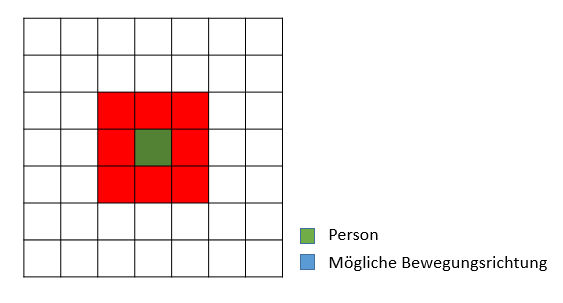
\includegraphics[width=0.5\textwidth]{abbildungen/MooreUmgebung.png}
	\caption{Moore-Umgebung}
	\label{fig:MooreUmgebung}
\end{figure}
\\
Die Personen können nur freie Zellen betreten. Jede Person wählt genau die Zelle als nächste Zelle, welche ihr den steilsten Nutzenanstieg ermöglicht. Der Nutzen der verschiedenen Zellen wird abhängig vom verwendeten Algorithmus unterschiedlich berechnet. Darüber hinaus soll der Nutzen durch die Position der anderen Personen beeinflusst werden. \\

Hierfür wird zwischen zwei Bereichen, abhängig vom Abstand zur nächsten Person unterschieden. Beträgt der Abstand zu einer fremden Person weniger als $45cm$, wird der vertraute Bereich (intimate space) der Personen betreten. Beträgt der Abstand zwischen $45cm$ und $120cm$, wird der persönliche Bereich (personal space) der Personen betreten. Für den vertrauten Bereich ist der Nutzenverlust (Nv(x)), abhängig vom Abstand $x$, nach Funktion \ref{Equ:NutzenverlustV} definiert. Für den persönlichen Bereich wird der Nutzenverlust (Np(x)), wiederum abhängig vom Abstand $x$ zur anderen Person, durch die Funktion \ref{Equ:NutzenverlustP} definiert. 

\begin{equation}
\label{Equ:NutzenverlustP}
Np(x)= \mu * \exp(\frac{4}{(\frac{d(x)}{\delta_p * r})^{2} -1}) 
\end{equation}

\begin{equation}
\label{Equ:NutzenverlustV}
Nv(x)= Np + \frac{\mu}{a_p} * \exp(\frac{4}{(\frac{d(x)}{\delta_v * r})^{2*b_p} -1}) 
\end{equation}

$d(x)$ beschreibt den aktueller Abstand zur nächsten Person. Die folgende Tabelle enthält die Bedeutung der einzelnen Parameter und die entsprechenden Werte: 

\begin{table}[htpb]
	\centering
	\begin{tabular}{lll}
		Parameter & Beschreibung  &  Wert\\ \hline
		$\mu$ & Stärke des Nutzenverlustes & 5.0 \\
		$a_p$ & Dämpfung zwischen vertrautem und persönlichem Bereich & 1.0 \\
		$b_p$ & Stärke des Übergangs zwischen vertrautem und persönlichen Bereich &1 \\
		$\delta_p$ & persönlicher Bereich [m]& 1.20 \\
		$\delta_v$ & vertrauter Bereich [m]& 0.45 \\
		$r$ & Radius einer Person [m] & 0.2  
	\end{tabular}
	\caption{Parameter und Werte für die Berechnung des Nutzenverlustes}
	\label{tab:parameterNutzenverlust}
\end{table}

Der Radius einer Person sowie die Abstände für den vertrauten und persönlichen Bereich wurden auf Basis des Modells von Hall aus \cite{VONSIVERS2015104} übernommen. Weitere Erläuterungen zu den Parametern, den Werten und den verwendeten Funktionen sind im Kapitel \ref{Personenpotenzial} beschrieben.
 
\subsection{Geschwindigkeit der Personen}
Jede Person soll eine individuelle Wunschgeschwindigkeit besitzen. Sie bewegt sich bei freier Bahn mit dieser Geschwindigkeit fort. Die Wunschgeschwindigkeiten sollen als normalverteilt angesehen werden. Als Mittelwert und Standardabweichung sollen die errechneten Werte aus der ersten Studienarbeit verwendet werden.

\subsection{Zeitmodellierung}
Die Simulation unterliegt keinen harten Echtzeitanforderungen. Sie soll für die gesamte Simmulationsdauer so schnell wie möglich durchgeführt werden. Es soll keine globale Uhr modelliert werden. \\
Die Visualisierung der Simulation soll hingegen die Bewegungen der Personen möglichst in Echtzeit darstellen. Sie unterliegt weichen Echtzeitanforderungen. Abweichungen aufgrund mangelnder Rechner-Ressourcen sind tolerierbar. 

\subsection{Parameter}
Die Tabelle \ref{tab:parameter} zeigt alle möglichen Parameter, welche die Software steuern. Alle Parameter sind optional.
\begin{table}[htpb]
	\centering
	\begin{tabular}{lll}
		Parameter & Beschreibung  &  Default\\ \hline
		--free-flow-velocity & Mittelwert der Wunschgeschwindigkeit [m/s] & 1,0 \\
		--free-flow-deviation & Standardabweichung der Wunschgeschwindigkeiten [m/s] & 0 \\
		--algorithm & Algorithmus (euclid, dijkstra, fast-marching) & dijkstra \\
		--output-folder & Ordner in den der Output gespeichert wird & ../data/ \\
		--cellsize & Größe der einzelnen Zellen [m] & 1 \\
		--input-map & Pfad zum Bild der map (Auswahl des Testfalls) & ../defaultmap/default.png \\
		
	\end{tabular}
	\caption{Parameter und Defaultwerte}
	\label{tab:parameter}
\end{table}
	
\subsection{Berechnungen}
Die Aufgabe der Software ist die Simulation von Personenbewegungen. Für möglichst genaue Zeitangaben wird die Java Klasse BigDecimal verwendet. Für die Division werden 32 Nachkommastellen berücksichtigt und als Rundungsmodus wird Half\_Even verwendet, da dieser kumulative Fehler bei sich wiederholenden Berechnungen minimiert. Die anschließende Berechnung und Aufbereitung der Daten (insebesondere für den Test \ref{Anforderungen:RimeaTest}) erfolgt mit Mathematica.

\subsection{Report}
\label{Anforderungen:Report}
Alle errechneten Ergebnisse sollen über einen Report ausgeleitet werden. Für jedes Testszenario soll ein eigenes Verzeichnis angelegt werden, in dem der Report und die verwendete Map (vgl. Abschnitt \ref{AnforderungenTest}) gespeichert werden sollen. Der Report soll im .xml Format ausgeleitet werden um eine gute Weiterverarbeitung der Ergebnisse (Visualisierung) zu gewährleisten. Er soll alle benötigten Informationen, wie beispielsweise die einzelnen Events der Personen, die durch den Algorithmus berechneten Entfernungen der einzelnen Zellen vom Ziel und eine Übersicht über den Zustand der einzelnen Zellen (Fieldmap), für Simulation beinhalten. \\
Darüber hinaus sollen im Verzeichnis 3 .csv Dateien angelegt werden. Wird kein Messfeld (vgl. Abschnitt \ref{AnforderungenTest}) definiert, sollen diese nicht befüllt werden. Falls ein Messfeld in der Map definiert wurde, soll in der Datei $timeDensity.csv$ die Personendichte im Messbereich zu verschiedenen Messzeitpunkten gespeichert werden. In der Datei $timeVelocity.csv$ sollen die durchschnittliche Geschwindigkeit der Personen im Messbereich zu verschiedenen Messzeitpunkten gespeichert werden. Die Datei $fundamental.csv$ soll die ermittelten Personendichten und Geschwindigkeiten enthalten, sodass daraus bei Bedarf ein Fundamentaldiagramm erstellt werden kann. Messzeitpunkte sollen in einem Intervall von $0,5s$ definiert werden.\\

\subsection{Berechung des Zielnutzens}
\label{AnforderungenAlgorithmen}

Es sollen drei unterschiedliche Algorithmen für die Berechnung des Zielnutzens (Attraktivität) einer Zelle implementiert werden. \\
\\
Algorithmus 1: Der Nutzen bzw. die Attraktivität jeder Zelle entspricht dem negativen euklidischen Abstand. Hierbei können keine Hindernisse umgangen werden. Jede Person versucht den Nutzen zu maximieren und wählt jeweils die Zelle mit maximalen Wert aus den umliegenden aus.\\
\\
Algorithmus 2: Der Nutzen bzw. die Attraktivität jeder Zelle wird durch Floor-Flooding, basierend auf dem Dijkstra Algorithmus, berechnet. Für jede Zelle wird die geringste Anzahl an notwendigen Bewegungen bis zum Ziel ermittelt. \\
\\
Algorithmus 3: Analog zum Algorithmus 2 wird auch in diesem hier der Nutzen bzw. die Attraktivität jeder Zelle mittels Floor-Flooding berechnet. Es wird jedoch der Fast-Marching Alforithmus (Lösung der Eikonal-Gleichung) als Grundlage verwendet.

\subsection{Werte für die Auswertung}
Alle in der Tabelle \ref{tab:WerteAuswertung} aufgeführten Werte sollen auf Basis der Simulation ermittelt und ausgewertet werden. Einige Werte werden nur für bestimmte Tests benötigt.
\begin{table}[htpb]
	\centering
	\begin{tabular}{lll}
		Ermittelte Werte & Beschreibung & Wann benötigt\\ \hline
		mittlere Geschwindigkeit & durchschnittliche Geschwindigkeit & Rimea-Test 4\\
								 & der Personen im Feld &  \\	
		Fluss (Personen/Meter/s) & Anzahl der Personen mit Geschwindigkeit & Rimea-Test 4\\
								 & > 1m/s im Feld & \\
		Simulationsdauer & Dauer bis der Test beendet ist & bei allen Tests
	\end{tabular}
	\caption{Werte für die Auswertung}
	\label{tab:WerteAuswertung}
\end{table}

\subsection{Testszenarien für die Simulation}
\label{AnforderungenTest}

Die implementierten Algorithmen (vgl. Unterkapitel \ref{AnforderungenAlgorithmen} ) sollen anhand unterschiedlicher Testszenarien verglichen und verifiziert werden. Die verschiedenen Szenarien sollen der Simulation als .png Datei übergeben werden. 

\subsubsection{Erstellung der Testszenarien}
Es soll die Möglichkeit bestehen, unterschiedliche Testszenarien mittels eines Bildbearbeitungsprogrammes zu erstellen und an die Simulation (als .png Datei) zu übergeben. Bei der Erstellung ist sowohl die Anzahl der Personen, als auch die Anzahl der Hindernisse und Ziele (Personensenken) beliebig. Hinsichtlich der Farben der Objekte müssen jedoch die in der folgenden Tabelle \ref{tab:Farbcodes} beschriebenen Farbcodes verwendet werden. Jedes Pixel wird durch eine Zelle des Automaten repräsentiert. Darüber hinaus soll die Möglichkeit bestehen ein Messfeld zu definieren. In diesem Feld wird die durchschnittliche Geschwindigkeit der Personen ermittelt in einer .csv Datei ausgegeben. Für das Messfeld müssen in der .png Datei lediglich die beiden diagonalen Eckpunkte angegeben werden. Die Implementierung ermittelt die Koordinaten und erstellt daraus ein rechteckiges Feld. 
 
\begin{table}[htpb]
	\centering
	\begin{tabular}{lll}
		Farbcode & Farbe & Bedeutung\\ \hline
		\#3F48CC & Blau & Ziel/ Personensenke \\	
		\#000000 & Schwarz & Ziel/ Personensenke \\
		\#FFFFFF & Weiß & Leere Zelle \\
		\#22B14C & Grün & Person \\
		\#FF0000 & Rot  & Messfeld
	\end{tabular}
	\caption{Werte für die Auswertung}
	\label{tab:Farbcodes}
\end{table}
 
\subsubsection{Testszenario: Freier Fluss}
Im Zuge dieses Tests soll überprüft werden, ob sich Personen bei freier Bahn (keine Hindernisse zwischen Start und Ziel) mit ihrer jeweiligen Wunschgeschwindigkeit auf das Ziel hin bewegen. Des weiteren soll überprüft werden, ob die Person den kürzesten Weg verwendet. Der Test soll mit allen 3 Betriebsmodi durchgeführt werden. Abbildung \ref{fig:AnforderungenTest_FreierFluss} stellt den Testaufbau schematisch dar.

\begin{figure}[htpb]
	\centering
	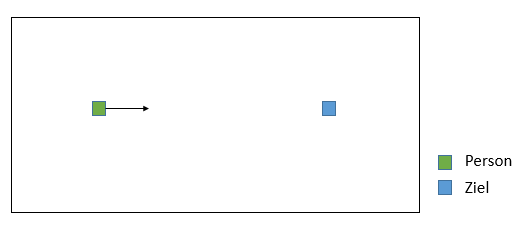
\includegraphics[width=0.8\textwidth]{abbildungen/Test_FreierFluss.png}
	\caption{Testfall Freier Fluss (schematisch)}
	\label{fig:AnforderungenTest_FreierFluss}
\end{figure}

\subsubsection{Testszenario: Hühnertest}
Zwischen Start und Ziel soll ein U-förmiges Hindernis (Öffnung in Richtung des Startes) eingefügt werden. Abhängig vom verwendeten Algorithmus wird ein unterschiedliches Ergebnis erwartet:\\
Euklid: Die Personen sollen sich auf dem kürzesten Weg auf das Ziel zubewegen. Sobald sie das Hindernis erreicht haben, sollen sie stehen bleiben. Erwartungsgemäß wird der Test nicht erfolgreich verlaufen. \\
Dijkstra und Fast-Marching Algorithmus: Die Personen sollen das Hindernis umgehen und das Ziel erreichen. Bei einem \glqq Feststecken im Hindernis\grqq (wie bei Verwendung des Euklid Algorithmus erwartet) wird der Test als fehlgeschlagen gewertet. Abbildung \ref{fig:AnforderungenTest_Hühner} stellt den Testaufbau schematisch dar.

\begin{figure}[htpb]
	\centering
	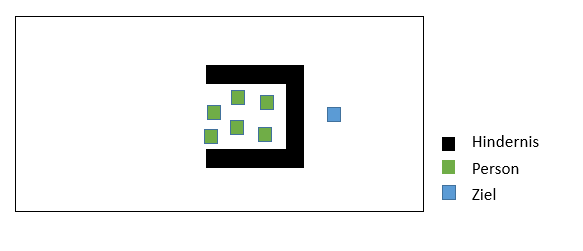
\includegraphics[width=0.8\textwidth]{abbildungen/Test_Huehner.png}
	\caption{Testfall Hühnertest (schematisch)}
	\label{fig:AnforderungenTest_Hühner}
\end{figure}
 
\subsubsection{Testszenario: Evakuierung eines Raumes mit 2 Türen}
\label{Anforderungen:Evakuierung2}
Die Personen befinden sich zu Beginn in einen von Hindernissen umgebenen, quadratischen Raum. An 2 Seiten sind Öffnungen platziert (freie Zellen). Hinter diesen Öffnungen befinden sich jeweils Ziele. Im Laufe des Tests sollen die Personen durch die beiden Engstellen zum Ziel gelangen. \\
Dieser Test soll auf Basis des Dijkstra und Fast-Marching Algorithmus in unterschiedlichen Versionen durchgeführt werden. Zunächst sollen die Türen an benachbarten Seiten mit sehr geringem Abstand zueinander platziert werden. Anschließend sollen die Türen an gegenüberliegenden Seiten mit sehr großem Abstand zueinander platziert werden. Unterschiede hinsichtlich der Evakuierungsdauer, aufgrund der Algorithmen oder Positionen der Türen sind festzuhalten. Die Abbildung \ref{fig:AnforderungenTestEvak2TürNebeneinander} zeigt die unterschiedlichen Testversionen schematisch.

\begin{figure}[!htb]
	\centering
	\begin{minipage}{.5\textwidth}
		\centering
		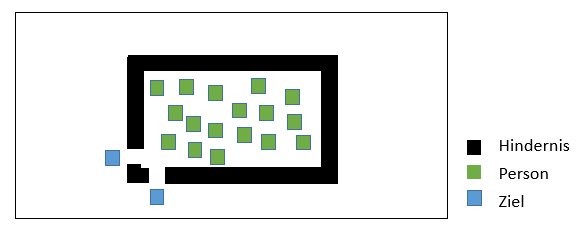
\includegraphics[width=\textwidth]{abbildungen/Test_Evakuierung2_Nebeneinander.png}
	\end{minipage}%
	\begin{minipage}{0.5\textwidth}
		\centering
		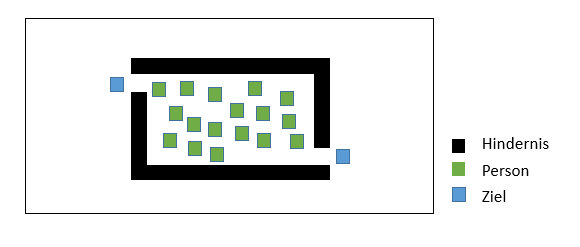
\includegraphics[width=\textwidth]{abbildungen/Test_Evakuierung2_NebeneinanderMax.png}
	\end{minipage}
	\label{fig:AnforderungenTestEvak2TürNebeneinander}
	\caption{Testfall Evakuierung eines Raumes mit 2 Türen, links: geringer Abstand zwischen den Türen, rechts: großer Abstand zwischen den Türen}
\end{figure}

\subsubsection{Testszenario: Evakuierung eines Raumes mit 4 Türen}
Für diesem Testfall soll sich an jeder Raumseite eine Tür befinden. Der Raum soll absolut symmetrisch aufgebaut sein und die Türen sollen sich jeweils in der Mitte jeder Raumseite befinden. In einem weiteren Szenario sollen zwei Türen an gegenüber liegenden Seiten entfernt werden. Ziel dieser beiden Testszenarien soll es sein, die Unterschiede hinsichtlich der Evakuierungsdauer eines identischen Raumes zu ermitteln, wenn sich in diesem zwei oder vier Türen befinden. Die Simulation soll anhand dieses Aspekts verifiziert werden. Es wird erwartet, dass sich die Evakuierungszeit durch die doppelte Anzahl an Türen nahezu halbiert.

\subsubsection{Testszenario: Fundamentaldiagramm - Rimea-Test 4}
\label{Anforderungen:RimeaTest}
In diesem Testfall soll ein $65m$ langer und $12m$ breiter Gang angelegt werden. Auf der einen Seite des Ganges befindet sich die Personenquelle, auf der anderen Seite die Personensenke. Im Laufe des Testes sollen die Personen den Gang entlangschreiben. Die Anzahl der Personen ist zu variieren. In einer weiteren Version des Tests sollen Personen, welche die Personensenke erreicht haben, erneut bei der Personenquelle starten (Endlosschleife). Abbildung \ref{fig:Test_Rimea4} zeigt den Testaufbau schematisch.

\begin{figure}[htpb]
	\centering
	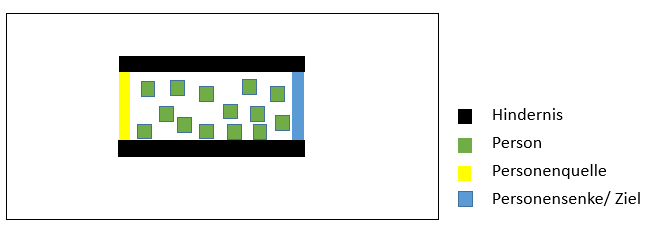
\includegraphics[width=0.8\textwidth]{abbildungen/Test_Rimea4-2.png}
	\caption{Testfall Rimea 4 (schematisch)}
	\label{fig:Test_Rimea4}
\end{figure}

\subsubsection{Testszenario: Engstelle (unidirektional)}
In diesem Testfall soll ein $72\ m$ langer und $11,6\ m$ breiter Gang angelegt werden. Am Ende des Ganges befindet sich eine Engstelle mit $1,2\ m$ Breite und dahinter die Personensenke. Es soll mit variierender Anzahl an Personen getestet werden, wie lange es dauert bis die Personen im Ziel (bzw. in der Personensenke) angekommen sind. Der schematische Testaufbau ist in Abbildung \ref{fig:Engstelle} aufgeführt.

\begin{figure}[htpb]
	\centering
	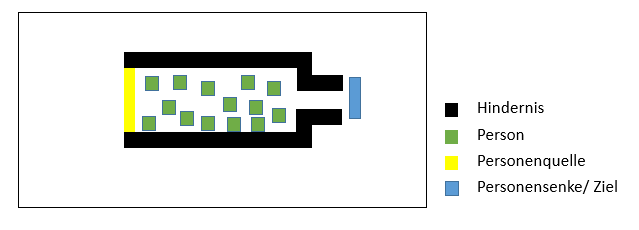
\includegraphics[width=0.8\textwidth]{abbildungen/Test_Engstelle.png}
	\caption{Testfall Engstelle (schematisch)}
	\label{fig:Engstelle}
\end{figure}

\subsection{Visualisierung}

Die Visualisierung soll die errechneten Personenbewegungen graphisch darstellen. Als Grundlage soll der ausgegebene Report (vgl. Abschnitt \ref{Anforderungen:Report}) dienen. Konkrete Anforderungen bezüglich der Visualisierung sind in Abbildung \ref{fig:AnforderungenVisualisierung} abgebildet.

\begin{figure}[htpb]
	\centering
	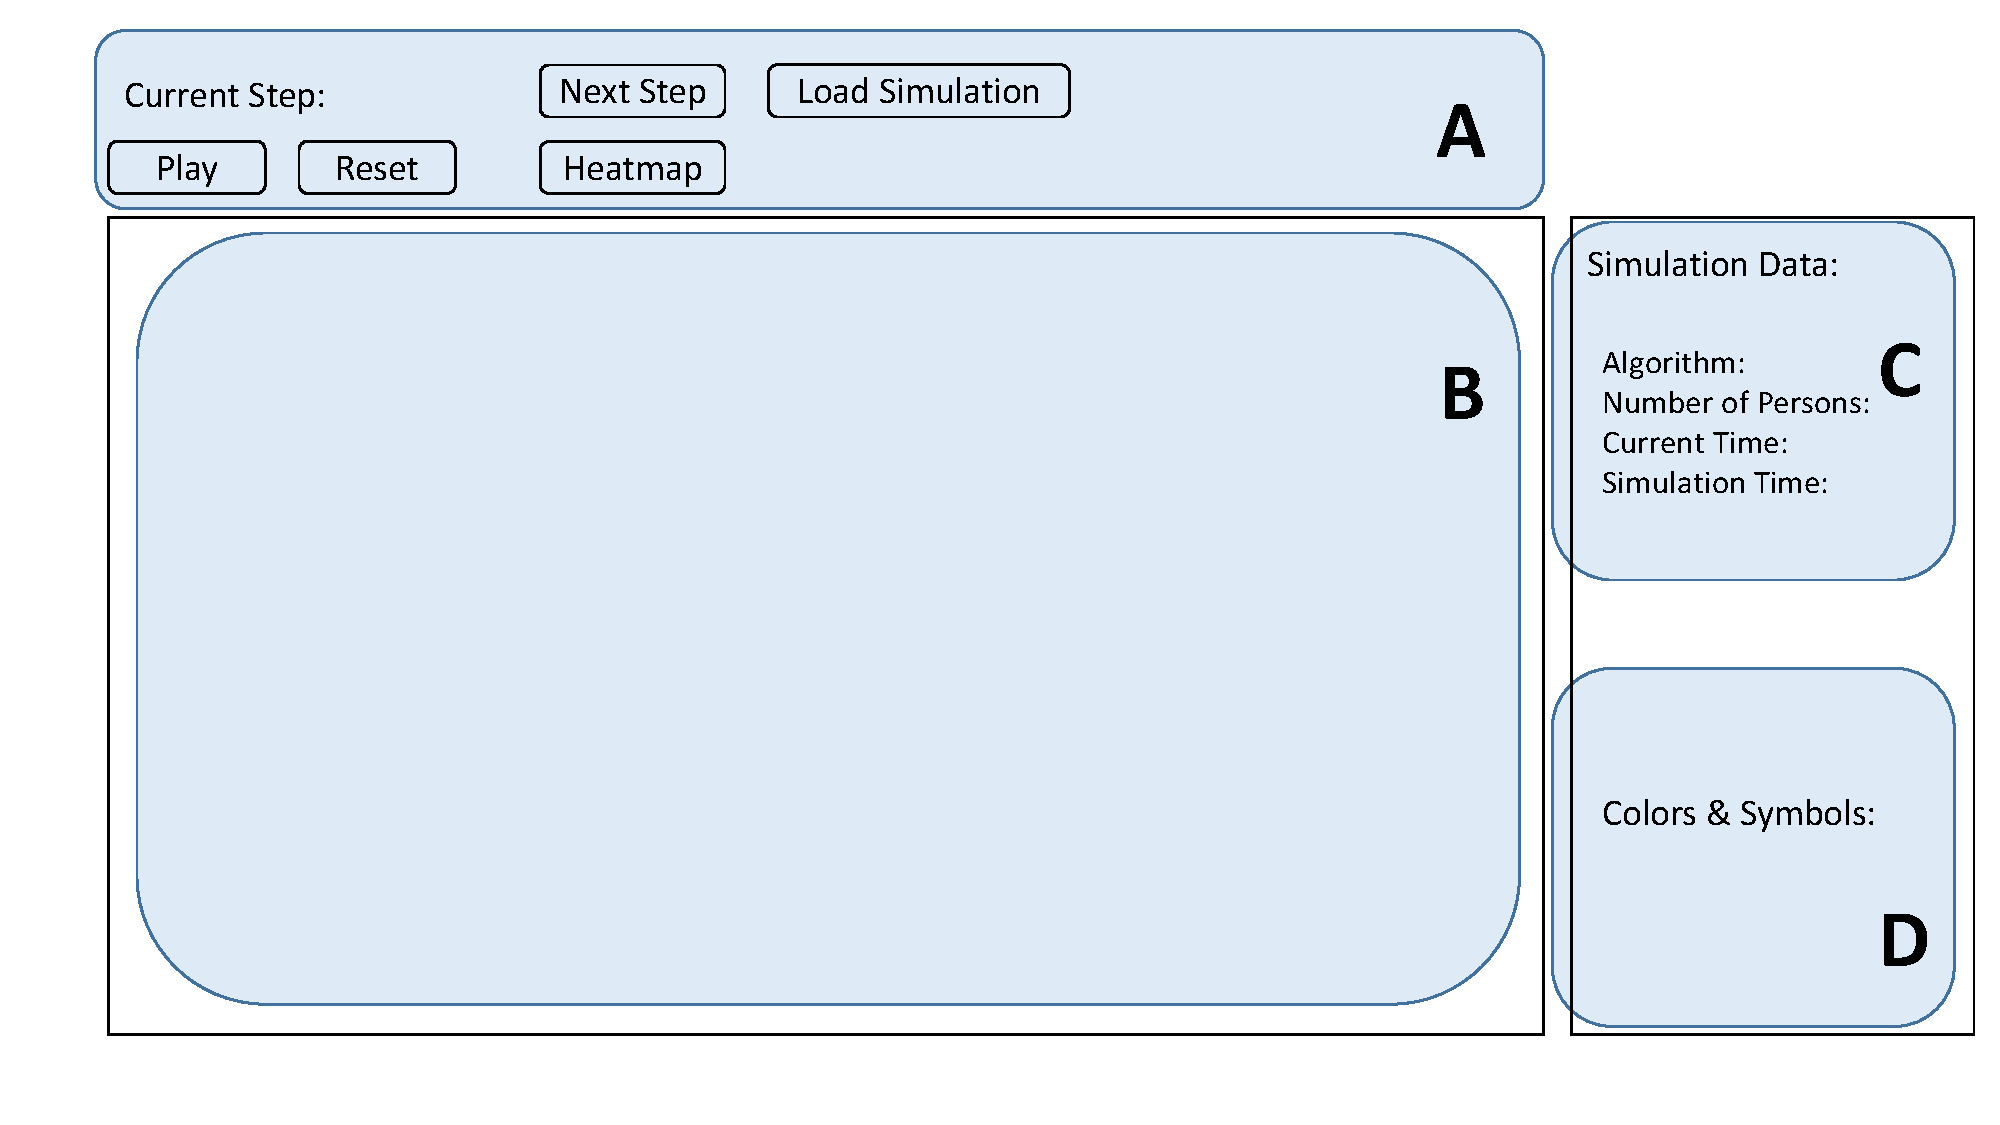
\includegraphics[width=0.8\textwidth]{abbildungen/AnforderungenVisualisierung.pdf}
	\caption{Visualisierung (schematisch)}
	\label{fig:AnforderungenVisualisierung}
\end{figure}

Die Oberfläche der Visualisierung soll aus 4 verschiedenen Teilen bestehen, welche in der Abbildung durch die blauen Kästen A-D hervorgehoben wurden. Im Teil A sollen Konfigurationsmöglichkeiten für die Visualisierung aufgeführt sein. Beispielsweise soll zwischen einer normalen Darstellung der Simulation und einer Heatmap gewechselt werden können. Darüber hinaus soll die Möglichkeit bestehen, die Visualisierung zu stoppen und schrittweise fortzusetzen. \\
Teil B enthält die eigentliche Visualisierung der Personen, Hindernisse und Ziele. In Teil C sind alle Informationen bezüglich der Visualisierung aufgeführt und Teil D enthält eine Legende der verwendeten Symbole und Farben. Wird ein Messfeld definiert, soll dieses in der Visualisierung hervorgehoben werden.


\section{Beeinflussung durch andere Personen} 
\label{Personenpotenzial}

Wie bereits im Abschnitt \ref{Anf:Personen} kurz erläutert, wird die Entscheidung, welche Zelle eine Person als nächstes betritt abhängig vom verwendeten Algorithmus und von den Positionen der anderen Personen getroffen. In der Realität fühlen sich Personen unwohl, wenn sie anderen, insbesondere fremden Personen zu nahe kommen. Sie versuchen folglich eine solche Situation wenn möglich zu vermeiden. Beispielsweise bei der Fahrt in einem überfüllten Aufzug lässt sich diese Situation unter Umständen nicht vermeiden. Bei der Fortbewegung in der Ebene jedoch häufig schon. Personen neigen in der Realität dazu einen Umweg in kauf zu nehmen, um einem Gedränge zu entkommen. Um dieses Verhalten in der Simulation zu berücksichtigen existieren verschiedene mathematische Funktionen, mithilfe derer ein Abstoßungspotenzial berechnet wird. Während auf der einen Seite der Nutzen einer Person steigt, je näher sie dem Ziel kommt, verringert sich dieser Nutzen auf der anderen Seite wieder, wenn sie anderen Personen zu nahe kommen. Mit Hilfe von Funktionen kann somit der Nutzenverlust einer Person bestimmt werden. \\
Insbesondere glatte Funktionen auf kompakten Trägern, die außerhalb eines begrenzten Gebietes komplett zu verschwinden (f(x) = $0$) eignen sich hierfür gut. Würde man eine Funktion verwenden, deren Funktionswert auch außerhalb des begrenzten Gebietes größer als $0$ ist, führe dies zu einer Abweichung von der Realität und damit zu einem Fehler. In diesem Fall, wird eine Person im Modell auch durch eine sehr weit entfernte Person, wenn auch nur leicht, beeinflusst. Dies widerspricht der Realität, da das Abstoßungspotenzial von Personen auf einen Bereich um die entsprechende Person beschränkt ist. \\
In der Fachliteratur wird beispielsweise folgende Funktion vorgeschlagen:
\begin{displaymath}
\label{equ:NutzenverlustSCHLECHT}
N(d) = 
\left\{ 
\begin{array}{cc}
-h \exp(\frac{1}{(\frac{d}{w})^2 -1}) & \;\;\;\;\;\;\;\;\;\;\; falls\, |d| < w  \\
0 & sonst  
\end{array} 
\right.
\end{displaymath}
Hierbei wird der Nutzenverlust ($N(d)$), abhängig vom Abstand $d$ zur nächsten Person definiert. $w$ beschreibt die Reichweite der Funktion und $h$ die Stärke der Beeinflussung bzw. des Nutzenverlustes \cite{DIETRICH2014841}. \\ 
Für die Ermittlung des Abstoßungspotenzials bzw. des Nutzenverlustes aufgrund anderer Personen wurden jedoch anstelle dieser Funktion, die in Abschnitt \ref{Anf:Personen} aufgeführten Funktionen \ref{Equ:NutzenverlustP} und \ref{Equ:NutzenverlustV} verwendet. Diese basieren auf dem Modell von Hall, das den Bereich um eine Person in mehrere Teilbereiche einteilt. In einem Umkreis von bis zu $45cm$ wird der vertraute Bereich einer Person betreten. Befinden sich zwei Personen so nah beieinander, können Berührungen nicht vermieden werden. Zwischen $45cm$ und $120cm$ um eine Person befindet sich der persönliche Bereich, welcher beispielsweise von Freunden oder Familienmitgliedern betreten werden darf. Ein Betreten dieses Bereichs durch fremde Personen wird als unangenehm und aufdringlich empfunden und Personen versuchen es folglich zu vermeiden. Darüber hinaus definiert Hall noch zwei weitere Bereiche. Zwischen $120cm$ und $360cm$ um die Person befindet sich der soziale oder gesellschaftliche Bereich der Person und ab $360cm$ der öffentliche Bereich. Für die Simulation in dieser Studienarbeit sind die beiden letzten Bereiche jedoch nicht relevant, da der Einfluss auf den Nutzen der Person zu gering ist, um die Entscheidung, wohin die Person als nächstes geht zu beeinflussen. Außerdem lässt sich das Betreten dieser beiden Bereiche durch andere Personen bei einer höheren Personendichte generell nicht vermeiden.\\
Hintergrund dieser Entscheidung ist, dass nach unserer Einschätzung und nach \cite{VONSIVERS2015104} die Berücksichtigung des Modells von Hall durch die Verwendung unterschiedlicher Funktionen für den vertrauten und persönlichen Bereich zu einem Verhalten, das der Realität näher kommt, führt. Berührt eine Person eine fremde Person, fühlt sie sich deutlich unwohler, als wenn sie dieser lediglich nahe kommt mit einem Abstand von beispielsweise $50cm$. Diese Eigenschaft wird durch die Funktion \ref{equ:NutzenverlustSCHLECHT} kaum berücksichtigt.\\
Außerdem lassen sich in dieser Simulation, durch die Wahl einer geringen Zellgröße des zellulären Automatens von $40 cm$, die Auswirkungen der unterschiedlichen Bereiche auf den Nutzenverlust bzw. das Abstoßungspotenzial der Personen feststellen. \\
Darüber hinaus beinhalten die Funktionen \ref{Equ:NutzenverlustP} und \ref{Equ:NutzenverlustV} deutlich mehr Parameter. Diese Parameter können an mögliche gesellschaftliche oder länderspezifische Unterschiede angepasst werden und so die Realität besser widerspiegeln. Für diese Studienarbeit wurden die Parameter wie in der Tabelle \ref{tab:parameterNutzenverlust} aufgeführt gewählt. Grundlage hierfür sind die in \cite{VONSIVERS2015104} erläuterten Erkenntnisse aus unterschiedlichen Versuchen. Außerdem zeigten mehrere, in der Gruppe durchgeführten Simulationen mit unterschiedlichen Parameterkombinationen, dass sich das Abstoßungspotenzial durch die Verwendung dieser Parameter so auswirkte, wie man es in der Realität erwarten würde. \\ 
  
%TODO: VERSUCH DER DAS BEWEIST EINFÜGEN

\section{Softwaredesign}

Der Aufbau der Anwendung wurde im Team diskutiert und anschließend mittels UML spezifiziert.


\section{Softwaretest}


\section{Vergleich der Algorithmen}
\subsection{Euklid}
\subsection{Dijkstra}
\subsection{Fast Marching}




\section{Einfluss der Zellgröße auf die Abstandsberechnung}
Bei der Berechnung der Abstände hat die Wahl der Zellgröße je nach Algorithmus einen entscheidenden Einfluss auf die Ergebnisse der Simulation. Die Zellgröße gibt nicht nur die minimale Schrittweite vor, sondern hat auch Einfluss auf die Genauigkeit der Nutzenberechnungen. Um einen Vergleich darzustellen wurde ein Quadratisches Feld angelegt. Die Zellgröße des Feldes sowie die Anzahl der Felder wurden so variiert, dass die Entfernung von der rechten unteren Ecke zur linken oberen Ecke (am weitesten entfernter Punkt) immer den gleichen Abstand hat. Es wird also die Diagonale des Rechtecks berechnet. Die Abbildung \ref{fig_euklid_fast_marching_2m_cellsize} Zeigt den Vergleich beider Algorithmen bei der der Abstandsberechnung. Üblicherweise wird die Rabskala so gewählt um alle Werte vom kleinsten Abstand zum weitesten Punkt abzubilden. Um den Vergleich an dieser Stelle deutlich zu machen, wurde für beide Bilder die selbe Farbskala verwendet. Mit Bloßem Auge ist die Differenz nur schwer zu erkennen. Es ist jedoch sichtbar, dass das Feld, welches mit dem Euklid algorithmus berechnet wurde, einen deutlicheren Bogen aufweist. 

Eine Möglichkeit die Unterschiede zu visualisieren ist es, die Bilder mittels einer Differenzbildung der Beiden Bilder. Dafür wird ein Bild als Basis hergenommen und das zweite Bild als eine Ebene darber eingefügt. Die Farben der zweiten Ebene werden von der ersten Ebene Subtrahiert. Gleichen sich die Farben beider Ebenen, so ist das Ergebnis schwarz. Dieser Vergleich macht nur Sinn, wenn für beide Darstellungen die selbe Farbskala verwendet wurde, also die Entfernungen mit dem gleichen Farbcode codiert wurden. Die Abbildung \ref{fig_fast_marching_euclid_difference} zeigt die Differenzmenge der in Abildung \ref{fig_euklid_fast_marching_2m_cellsize} dargestellten Karten.
An diesem Bild ist deutlich zu erkennen, dass die Zellen, welche sich nur in X und nur in Y Richtung vom Ziel entfernen schwarz sind.  Es gibt also keinen Unterschied zwischen dem Euklidischen Abstand und dem Abstand welcher mittels Fast Marching berechnet wurde, bei einer Betrachtung der Zellen nur in X oder nur in Y Richtung. Entfernt man sich schräg vom Ziel (Also X und Y Anteil gleichzeitig), sieht man deutlich Differenzen der beiden Algorithmen.


Die Tabelle \ref{tab_euklid_fm_vergleich} zeigt die Ergebnisse dieses Experiments. Die Cellsize gibt dabei die Kantenlänge einer quadratischen Zelle an. Wichtig ist der Wert „Distance in X and Y“, welcher besagt, dass das Ziel in X und in Y Richtung immer jeweils 14 Zellen entfernt ist.
Nach der Formel wurde der Abstand von Ziel zum am weitesten entfernten Punkt berechnet:

$$a = \sqrt[]{x^2 +y^2} = \sqrt[]{(14\ m) ^2 +(14\ m) ^2} = 19,799\ m$$ 

Wie in der Tabelle zu sehen ist, berechnet der Euklid Algorithmus den Abstand sehr präzise. Da der Euklid Algorithmus kein „Gedächtnis“ hat also ohne Einfluss vorheriger Zellen berechnet und die oben genannte Formel anwendet ist der Algorithmus gut geeignet um die exakte Entfernung zu berechnen. Interessant in der Tabelle ist vor allem die Abweichung von 1,45 m, welche beim Fast Marching Algorithmus entsteht. Diese Abweichung entspricht einem Fehler von von 7,3 \% bezogen auf die tatsächliche Entfernung. Verringert man die Zellgröße, so konvergiert der Fast Marching Algorithmus gegen den euklidischen Abstand und der Fehler gegen 0. Die prozentualen Fehler in Abhängigkeit der Zellgröße sind in Abbildung \ref{fig_fast_marching_error_cellsize} dargestellt. 

\section{Einfluss der Zellgröße auf die maximale Dichte}
Darüber hinaus hat die Zellgröße direkten Einfluss auf die Dichte [$\frac{Personen}{m^2}$] in einem Feld. Würde man die Zellgröße von $2\ m^2$ wählen, erhielte man eine maximale Dichte von 0,5 $\frac{1}{m^2}$. Es ist darauf zu achten, dass die Zellgröße angemessen gewählt wird. Bei weiteren Versuchen wurde stets eine Zellbreite von 0,4 bis 0,5 m verwendet, sofern nichts anderes angegeben.



\begin{figure}
\centering
\begin{minipage}{.44\textwidth}
\centering
  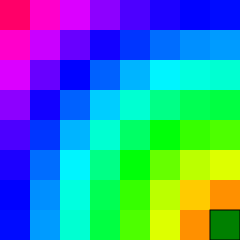
\includegraphics[width=0.9\linewidth]{abbildungen/vergleich_euklid_fast_marching/eEuclid_2m.png}
\end{minipage}%
\begin{minipage}{.44\textwidth}
\centering
  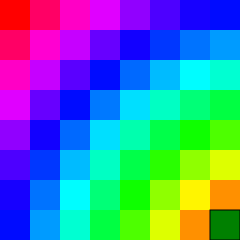
\includegraphics[width=0.9\linewidth]{abbildungen/vergleich_euklid_fast_marching/eFastMarching_2m.png}
\end{minipage}
\begin{minipage}{.1\textwidth}
\centering
  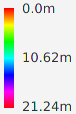
\includegraphics[width=\linewidth]{abbildungen/vergleich_euklid_fast_marching/farbskala.png}
\end{minipage}
\caption{Berechnung der Abstände mittels Euklid (links) und Fast Marching (rechts) an einem Feld mit einer Zellbreite von 2\ m. Dunkelgrün: Ziel, Rot: am weitesten entfernter Punkt im Feld}
\label{fig_euklid_fast_marching_2m_cellsize}
\end{figure}



\begin{figure}[ht]
	\centering
  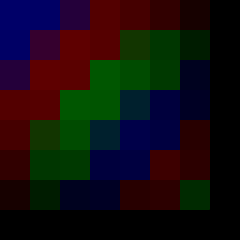
\includegraphics[width=0.4\textwidth]{abbildungen/vergleich_euklid_fast_marching/differenz_euklid_fast_marching.png}
	\caption{Differenzbildung der beiden Karten Euklid und Fast Marching}
	\label{fig_fast_marching_euclid_difference}
\end{figure}



\begin{table}[htbp]
\begin{tabular}{|l|r|r|r|r|r|r|r|}
\hline
Cellsize [m] & 2 & 1 & 0,5 & 0,25 & 0,125 & 0,0625 & 0,03125 \\ \hline
Cells in X and Y & 7 & 14 & 28 & 56 & 112 & 224 & 448 \\ \hline
Distance in  & & &  & &  & &\\ X and Y [m] & \textbf{14} & \textbf{14} & \textbf{14} & \textbf{14} & \textbf{14} & \textbf{14} & \textbf{14} \\ \hline
Tatsächliche & & &  & &  & &\\Entfernung [m] & 19,799 & 19,799 & 19,799 & 19,799 & 19,799 & 19,799 & 19,799 \\ \hline
Euklid [m] & 19,799 & 19,799 & 19,799 & 19,799 & 19,799 & 19,799 & 19,799 \\ \hline
Fast  & & &  & &  & &\\ Marching [m] & \textbf{21,245} & \textbf{20,717} & \textbf{20,363} & \textbf{20,137} & \textbf{19,997} & \textbf{19,913} & \textbf{19,863} \\ \hline
Diff [m] & 1,45 & 0,92 & 0,5645 & 0,3380 & 0,1979 & 0,1138 & 0,0644 \\ \hline
 & \multicolumn{1}{l|}{} & \multicolumn{1}{l|}{} & \multicolumn{1}{l|}{} & \multicolumn{1}{l|}{} & \multicolumn{1}{l|}{} & \multicolumn{1}{l|}{} & \multicolumn{1}{l|}{} \\ \hline
Error [\%]  & & &  & &  & &\\ diff/distance & \textbf{7,30} & \textbf{4,64} & \textbf{2,85} & \textbf{1,71} & \textbf{1,00} & \textbf{0,57} & \textbf{0,33} \\ \hline
\end{tabular}
\caption{Vergleich der Algorithmen Fast Marching und Euklid. Cellsize ist die Kantenlänge einer quadratischen Zelle in m (Zellbreite)}
\label{tab_euklid_fm_vergleich}
\end{table}


\begin{figure}[ht]
	\centering
  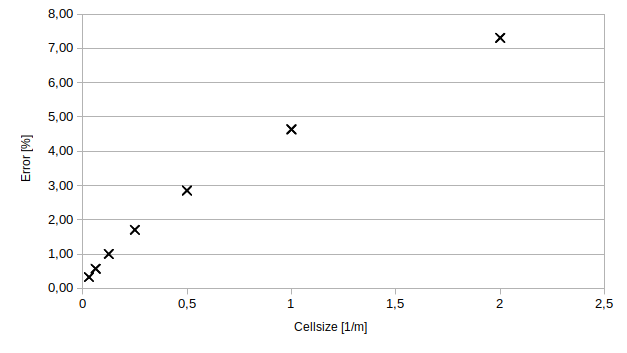
\includegraphics[width=\textwidth]{abbildungen/vergleich_euklid_fast_marching/fehler_zellgroesse.png}
	\caption{Prozentualer Fehler des Fast Marching Algorithmus in Abhängigkeit der Zellbreite}
	\label{fig_fast_marching_error_cellsize}
\end{figure}





\subsection{Verifikation}

\subsubsection{Verteilung Wunschgeschwindigkeit in der Ebene}
Um die korrekte Funktion der Simulation gewährleisten zu können, muss die Geschwindigkeit der Personen normal verteilt sein. Für die Überprüfung wurden die erzeugten Geschwindigkeiten von Fußgängern mitgeloggt und in einem Histogramm, das in Abbildung \ref{fig:Verteilung_Geschwindigkeit} zu sehen ist, dargestellt. Da die Werte sehr nah an der erwarteten Linie (in der Abbildung blau) liegen kann von einer Normalverteilung ausgegangen werden.

\begin{figure}[htpb]
	\centering
	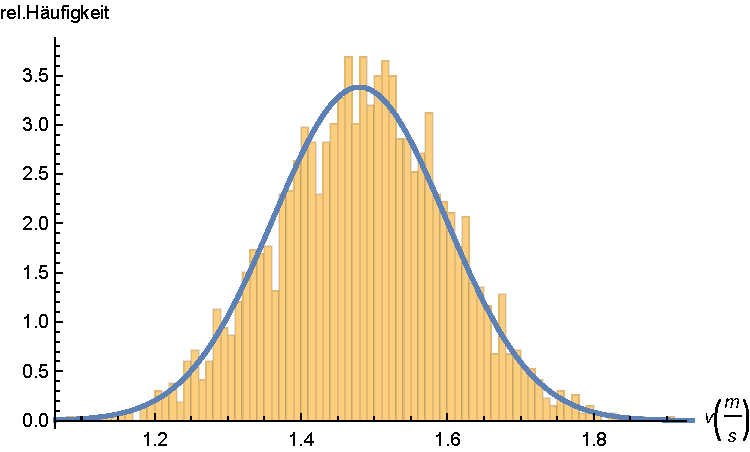
\includegraphics[width=0.5\textwidth]{abbildungen/histogramm.pdf}
	\caption{Verteilung der Geschwindigkeiten von Personen}
	\label{fig:Verteilung_Geschwindigkeit}
\end{figure}  

Dadurch, dass die Normalverteilung nicht das Thema dieser Arbeit ist, wurde von weiteren Tests auf Normalverteilung abgesehen.

In der Simulation ist es möglich einen Seed für die Geschwindigkeiten einzustellen um sicherzugehen, dass bei verschiedenen Durchläufen, die gleichen Verteilung von Personengeschwindigkeiten erfolgt.

\subsubsection{Hühnertest}
Der Hühnertest wurde auf Basis des in Abbildung \ref{fig:HühnertestMap} aufgeführten Feldes durchgeführt. Die einzelnen Farben der einzelnen Elemente sind analog zu den in Tabelle \ref{tab:Farbcodes} beschriebenen gewählt. Personen werden grün, Hindernisse schwarz und das Ziel blau dargestellt. Da mit Hilfe dieses Testes lediglich überprüft werden soll, ob die Personen den Weg aus dem Hindernis finden, ist die Anzahl von $39$ simulierten Personen ausreichend. Der Test wurde dreimal durchgeführt. Zunächst wurde der Euklid Algorithmus, anschließend Dijkstra und zuletzt der Fast-Marching Algorithmus für die Berechnung des Zielnutzens verwendet.

\begin{figure}[htpb]
	\centering
	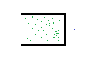
\includegraphics[width=0.5\textwidth]{abbildungen/HuehnertestMap.png}
	\caption{Ausgangsfeld des Hühnertests}
	\label{fig:HühnertestMap}
\end{figure}

Die Abbildungen \ref{fig:HühnerTestEuklidAnfang} und \ref{fig:HühnertestEuklidEnde} zeigen die Heatmap des Testes zu Beginn und am Ende des Testes auf Basis des Euklid Algorithmus. Wie zu erwarten war, laufen alle Personen im Verlauf des Tests auf dem kürzesten Weg in Richtung des Ziels. Sie sind nicht in der Lage das Hindernis zu Umlaufen und sammeln sich vor dem Hindernis, an der Stelle mit der geringsten Distanz zum Ziel. Dies wird durch die Heatmap verdeutlicht. Abhängig von der Farbe der Heatmap werden die unterschiedlichen Entfernungen der einzelnen Felder zum Ziel, und damit die Attraktivität der Felder dargestellt. Wie die Abbildungen zeigen, werden Hindernisse bei der Ermittlung der Entfernungen nicht berücksichtigt.
 
\begin{figure}[!htb]
	\centering
	\begin{minipage}{.5\textwidth}
		\centering
		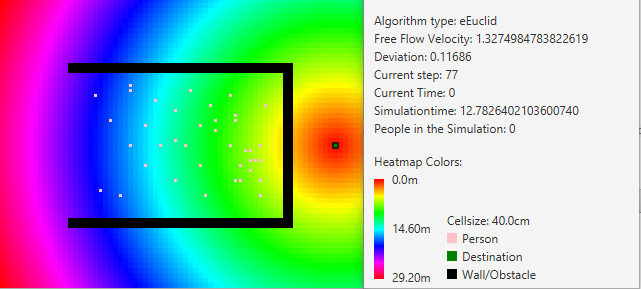
\includegraphics[width=\textwidth]{abbildungen/ChickenTest1BeginEuclid.PNG}
		\caption{Heatmap des Hühnertests mit dem Euklid Algorithmus (zu Beginn)}
		\label{fig:HühnerTestEuklidAnfang}
	\end{minipage}%
	\begin{minipage}{0.5\textwidth}
		\centering
		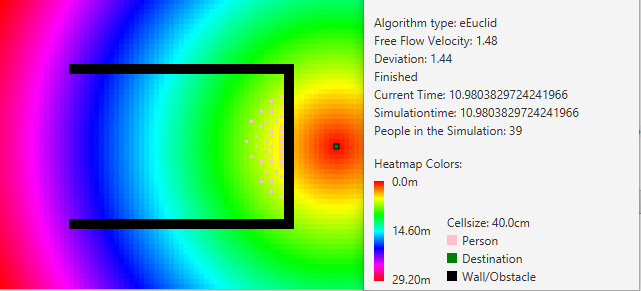
\includegraphics[width=\textwidth]{abbildungen/ChickenTest1EndEuclid.PNG}
		\caption{Heatmap des Hühnertests mit dem Euklid Algorithmus (Ende des Tests)}
		\label{fig:HühnertestEuklidEnde}
	\end{minipage}
\end{figure}

Im Vergleich dazu zeigen die Abbildungen \ref{fig:HühnerTestDijkstraAnfang} und \ref{fig:HühnertestDijkstraMitte} jeweils die Heatmap des Floor-Flooding mit dem Dijkstra Algorithmus zu Beginn der Simulation und nach einer SImulationsdauer von ca. $8s$. Es fällt auf, dass diese Heatmap deutlich anders aussieht, als die des Euklid Algorithmus. Die Hindernisse werden bei der Ermittlung der Entfernung der Zellen vom Ziel berücksichtigt und folglich farblich anders dargestellt. Abbildung \ref{fig:HühnertestDijkstraMitte} zeigt außerdem, dass sich die Personen in 2 Gruppen aufteilen und das Hindernis an beiden Seiten umlaufen. Nach einer Simulationsdauer von ca. $34,32s$ sind alle Personen im Ziel angekommen.

\begin{figure}[!htb]
	\centering
	\begin{minipage}{.5\textwidth}
		\centering
		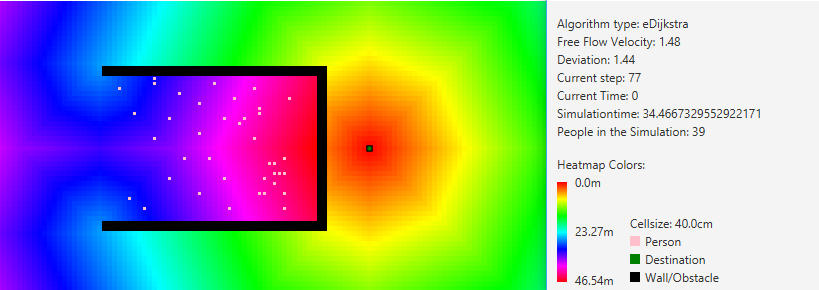
\includegraphics[width=\textwidth]{abbildungen/ChickenTestBeginDijkstra.PNG}
		\caption{Heatmap des Hühnertests mit dem Dijkstra Algorithmus (zu Beginn)}
		\label{fig:HühnerTestDijkstraAnfang}
	\end{minipage}%
	\begin{minipage}{0.5\textwidth}
		\centering
		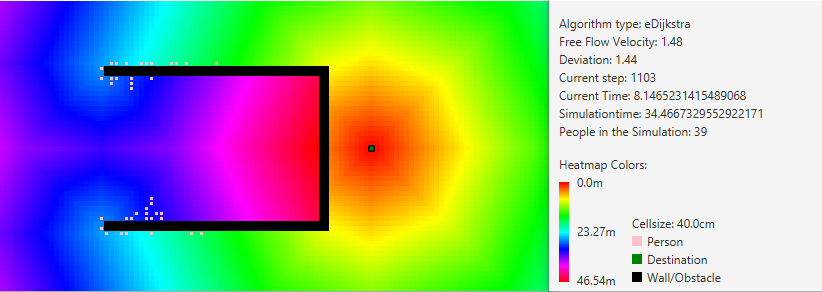
\includegraphics[width=\textwidth]{abbildungen/ChickenTestMitteDijkstra.PNG}
		\caption{Heatmap des Hühnertests mit dem Dijkstra Algorithmus (während der Simulation)}
		\label{fig:HühnertestDijkstraMitte}
	\end{minipage}
\end{figure}

Abschließend zeigt Abbildung \ref{fig:HühnertestFMAnfang} die Heatmap des Fast-Marching Algorithmus. 

\begin{figure}[htpb]
	\centering
	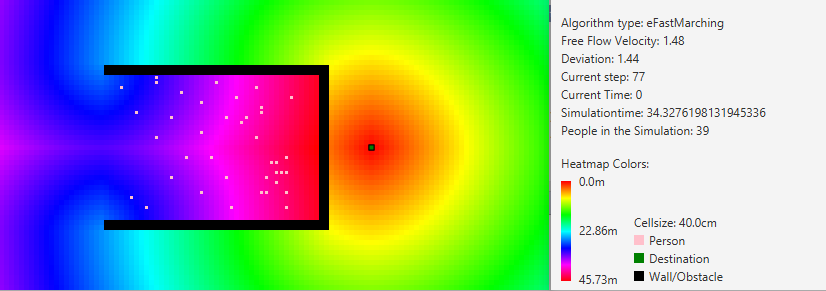
\includegraphics[width=0.5\textwidth]{abbildungen/ChickenTestBeginFM.PNG}
	\caption{Heatmap des Hühnertests mit dem Fast-Marching Algorithmus (zu Beginn)}
	\label{fig:HühnertestFMAnfang}
\end{figure}

Zusammenfassend ist festzustellen, dass die Personen in der Simulation mit dem Euklid Algorithmus im Hindernis hängen blieben. Bei den beiden anderen Algorithmen fanden sie den Weg ins Ziel. Beide Male teilten sie sich in 2 Gruppen auf. Für eine bessere Übersichtlichkeit wurde auf Abbildungen, welche das Ende des Tests mit dem Dijkstra bzw. Fast-Marching Algorithmus zeigen, verzichtet. Außerdem konnte festgestellt werden, dass die Simulationsdauer durch die Verwendung des Fast-Marching Algorithmus mit ca. $34,33s$ minimal kürzer als bei der Verwendung des Dijkstra Alogirithmus mit ca. $34,47s$ war.

\subsubsection{Evakuierung}
Mit Hilfe der verschiedenen Evakuierungstests sollen die Auswirkungen unterschiedlicher Positionen und Anzahl von Türen auf die Dauer der Evakuierung eines Raumes ermittelt werden. Die Berechnung des Zielnutzens auf Basis des Euklid Algorithmus wird hierbei nicht berücksichtigt. Dieser Algorithmus ist zwar gut geeignet um den kürzesten Weg zu einem Ziel zu finden, Hindernisse können jedoch nicht umgangen werden. Somit kann nicht ausgeschlossen werden, dass eine Person, beispielsweise in einer Ecke, \glqq hängen bleibt\grqq. Dieses Verhalten würde nicht der Realität entsprechen.

\paragraph{Evakuierung eines Raumes (Personen befinden sich in der Mitte)}
\label{EvaVerifikation}
Für die Verifikation der Simulation sollen sich die Personen zunächst alle dicht gedrängt, symmetrisch in der Mitte des Raumes befinden. An 2 gegenüberliegenden Seiten des Raumes soll sich jeweils eine Tür befinden (Evakuierung eines Raumes mit 2 Türen). In einer weiteren Simulation sollen sich an den anderen beiden Seiten jeweils eine weitere Tür befinden (Evakuierung eines Raumes mit 4 Türen). Die Evakuierungsdauer des Raumes mit 4 Türen müsste nun exakt halb so lange sein, wie die des Raumes mit 2 Türen. \\ 

Um eine möglichst symmetrische Anordnung der Personen sicher zu stellen, wurden alle Zellen des Raumes mit Personen belegt. Es wurden Evakuierungen mit $676$ Personen simuliert. Die beiden Räume, für die im weiteren Kapitel die Evakuierungszeiten verglichen werden, sind in Abbildung \ref{fig:Eva2T4TMap} dargestellt. Für die Evakuierungsdauer ist nicht die gesamte Simulationsdauer (Zeit bis die letzte Person das Ziel erreicht), sondern die Zeit, bis die letzte Person den Raum verlässt relevant. Dieser Bereich wurde in den Abbildungen mit einem roten Rahmen hervorgehoben. Alle Szenarien wurden zunächst auf Basis des Dijkstra Algortihmus simuliert. Die Abbildung \ref{fig:Eva2T4THeatMap} zeigt die Heatmap der Szenarien. Der symmetrische Nutzenanstieg in zwei bzw. vier Richtungen ist durch den Farbverlauf dargestellt. 

\begin{figure}[!htb]
	\centering
	\begin{minipage}{.5\textwidth}
		\centering
		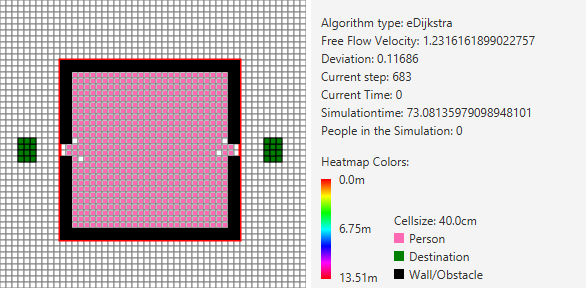
\includegraphics[width=\textwidth]{abbildungen/Evak2TuerenAnfang.png}
		
	\end{minipage}%
	\begin{minipage}{0.5\textwidth}
		\centering
		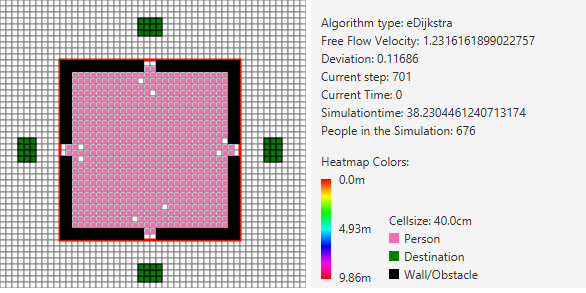
\includegraphics[width=\textwidth]{abbildungen/Evak4TuerenAnfang.png}
	\end{minipage}
	\caption{Evakuierung eines Raumes mit 2 Türen (links) und mit 4 Türen (rechts)}
	\label{fig:Eva2T4TMap}
\end{figure}

\begin{figure}[!htb]
	\centering
	\begin{minipage}{.5\textwidth}
		\centering
		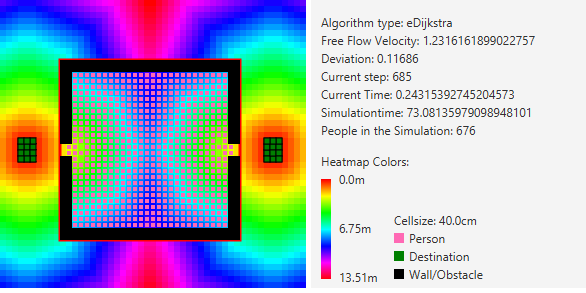
\includegraphics[width=\textwidth]{abbildungen/Evak2TuerenAnfangHeat.png}
	\end{minipage}%
	\begin{minipage}{0.5\textwidth}
		\centering
		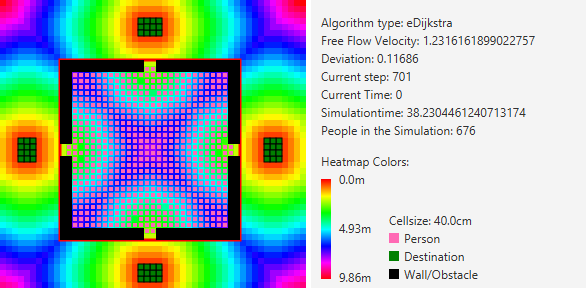
\includegraphics[width=\textwidth]{abbildungen/Evak4TuerenAnfangHeat.png}
	\end{minipage}
		\caption{Evakuierung eines Raumes mit 2 Türen (links) und mit 4 Türen (rechts), Heatmap}
		\label{fig:Eva2T4THeatMap}
\end{figure}

In Abbildung \ref{fig:Eva2T4TMitte} ist ein Ausschnitt der Simulationen nach einer Simulationszeit von ca. $24,1s$ (links) bzw. $15,5s$ (rechts) dargestellt. Es ist deutlich zu erkennen, dass sich jeweils ca. die Hälfte (2 Türen) bzw. ein Viertel der Personen (4 Türen) auf jede Tür zubewegen. 

\begin{figure}[!htb]
	\centering
	\begin{minipage}{.5\textwidth}
		\centering
		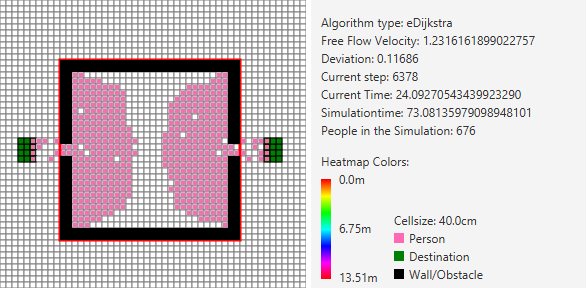
\includegraphics[width=\textwidth]{abbildungen/Evak2TuerenMitte.png}
	\end{minipage}%
	\begin{minipage}{0.5\textwidth}
		\centering
		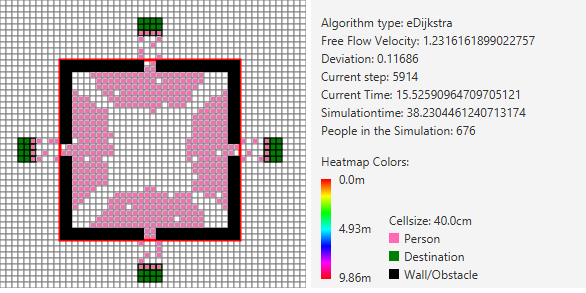
\includegraphics[width=\textwidth]{abbildungen/Evak4TuerenMitte.png}
	\end{minipage}
	\caption{Evakuierung eines Raumes mit 2 Türen (links) und mit 4 Türen (rechts), Ausschnitt}
	\label{fig:Eva2T4TMitte}
\end{figure}

Abschließend zeigt Abbildung \ref{fig:Eva2T4TEnde} die Evakuierungsdauer der beiden Räume. Die entsprechenden Ausschnitte zeigen den Moment, in dem die letzte Person den rot markierten Bereich verlassen hat. Bei der Simulation mit 2 Türen ist das nach ca. $73,07s$, bei der Simulation mit 4 Türen nach ca. $36,98s$. Durch die beiden zusätzlichen Türen verläuft die Evakuierung somit um das $1,98$ fache, also fast das $2$ fache schneller. Diese Übereinstimmung mit der Theorie kann als Indiz für die Richtigkeit der Simulation angesehen werden. \\

Die Abweichung ist zum einen dadurch zu erklären, dass die Geschwindigkeiten der Personen zufällig verteilt sind. Es kann also vorkommen, dass sich viele, etwas schneller gehende Personen im linken Teil des Feldes befinden und langsamer gehende rechts. Folglich würde die Evakuierung des linken Teils nicht so lange dauern, wie die des rechten und die anfängliche Symmetrie wäre nicht mehr vorhanden. Eine weitere Ursache könnte die Gestaltung der Implementierung sein. Eine Person, welche aktuell nicht ziehen kann (Felder mit größerem Nutzen als aktuell besetztes Feld sind belegt) wartet so lange, wie sie bräuchte um zum gewünschten Feld zu gehen, bis sie erneut versucht zu gehen. Das Verhalten ist unabhängig davon, ob das gewünschte Feld früher schon frei wird oder nicht. Somit warten Personen, obwohl sie theoretisch schon gehen könnten. 

\begin{figure}[!htb]
	\centering
	\begin{minipage}{.5\textwidth}
		\centering
		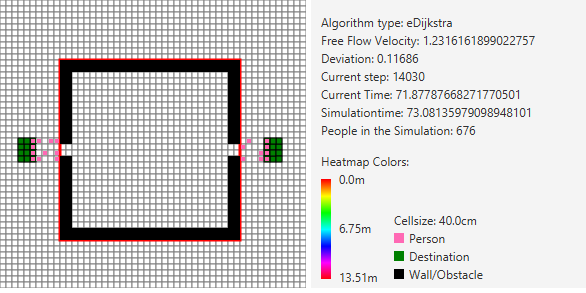
\includegraphics[width=\textwidth]{abbildungen/Evak2TuerenEnde.png}
	\end{minipage}%
	\begin{minipage}{0.5\textwidth}
		\centering
		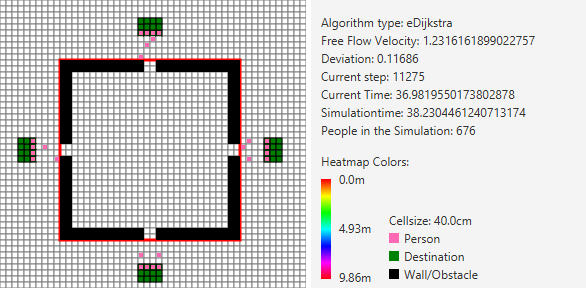
\includegraphics[width=\textwidth]{abbildungen/Evak4TuerenEnde.png}
	\end{minipage}
			\caption{Evakuierung eines Raumes mit 2 Türen (links) und mit 4 Türen (rechts), Ende der Evakuierung}
			\label{fig:Eva2T4TEnde}
\end{figure}

\begin{figure}[!htb]
	\centering
	\begin{minipage}{.5\textwidth}
		\centering
		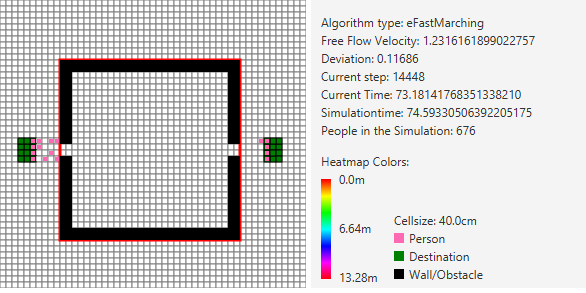
\includegraphics[width=\textwidth]{abbildungen/Evak2TuerenEndeFM.png}

	\end{minipage}%
	\begin{minipage}{0.5\textwidth}
		\centering
		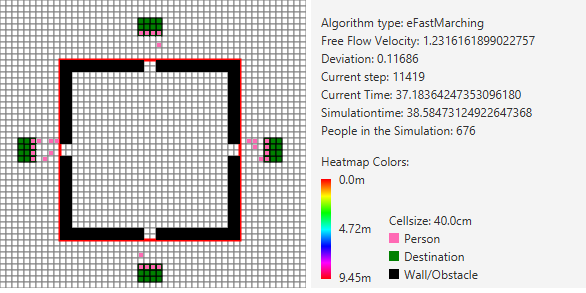
\includegraphics[width=\textwidth]{abbildungen/Evak4TuerenEndeFM.png}
	\end{minipage}
	\caption{Evakuierung eines Raumes mit 2 Türen (links) und mit 4 Türen (rechts), Fast-Marching Algorithmus (Ende der Evakuierung)}
	\label{fig:Eva2T4TEndeFM}
	\end{figure}

Zum Vergleich zeigt Abbildung \ref{fig:Eva2T4TEndeFM} die Evakuierungszeiten des identischen Raumes auf Basis des Fast-Marching Algorithmus. Auch hier ist die Dauer der Evakuierung bei zwei zusätzlichen Türen um den Faktor $1,97$ kürzer.\\

Stellt man die erläuterten Evakuierungsszenarien in Bezug zur Realität müssen einige Punkte beachtet werden. Zum einen befinden sich in der Realität niemals so viele Personen symmetrisch in einem Raum. Zum anderen ist es aufgrund von Brandschutz und anderen Sicherheitsvorgaben nicht zulässig $676$ Personen in einen ca. $108qm$ großen Raum zu lassen. Des weiteren wurden menschliche Faktoren wie Orientierungslosigkeit oder Panik in der Simulation nicht berücksichtigt. Die geringen Evakuierungszeiten sind überwiegend darauf zurückzuführen, dass jede Person zu jedem Zeitpunkt die perfekte Orientierung hat und genau die Zellen betritt, die auf dem für sie effizientesten Weg zum Ziel liegen. Diese Simulationen sind somit zusammenfassend als theoretisches Konstrukt zu sehen. Anhand dessen kann die Simulation gegen die Anforderung, dass sich die Evakuierungszeit bei Verdopplung der Türen Halbieren muss, verifiziert werden.

\paragraph{Evakuierung eines Raumes (Personen zufällig verteilt)}
In diesem Abschnitt werden weitere Evakuierungstests gegenübergestellt, bei denen die Personen zufällig im Raum verteilt wurden. Anhand dieser Tests sollen die Auswirkungen unterschiedlicher Positionen der Türen auf die Evakuierungsdauer simuliert werden.\\

\begin{figure}[htpb]
	\centering
	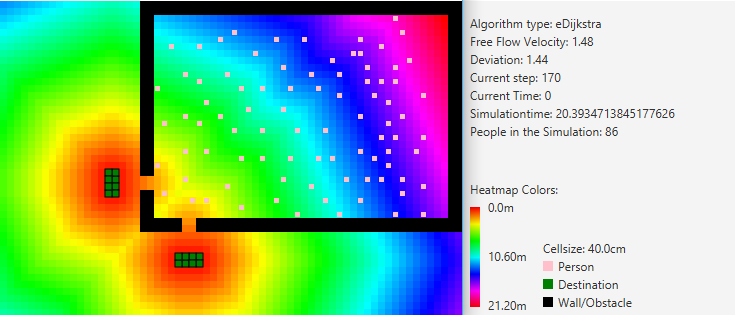
\includegraphics[width=0.8\textwidth]{abbildungen/Evak1DBegin.PNG}
	\caption{Verteilung der Personen (Heatmap Dijkstra Algorithmus)}
	\label{fig:EvakuierungMap}
\end{figure}

Abbildung \ref{fig:EvakuierungMap} zeigt die Verteilung der Personen, die für unterschiedliche Evakuierungstests verwendet wird. Somit wird eine bessere Vergleichbarkeit der Ergebnisse erzielt. In der Abbildung ist außerdem die Heatmap des Dijkstra Algorithmus für dieses Szenario zu sehen. 

\begin{figure}[!htb]
	\centering
	\begin{minipage}{.5\textwidth}
		\centering
		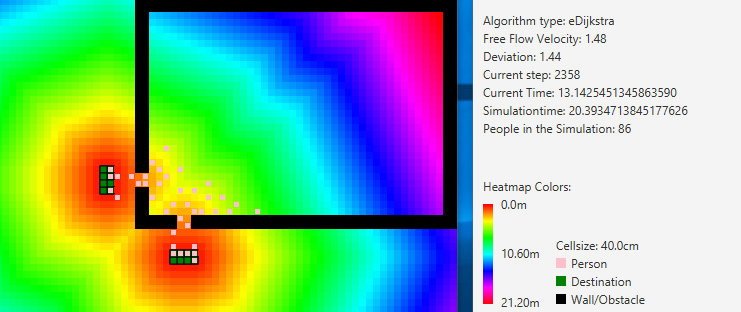
\includegraphics[width=\textwidth]{abbildungen/Evak1DMitte.PNG}
	\end{minipage}%
	\begin{minipage}{0.5\textwidth}
		\centering
		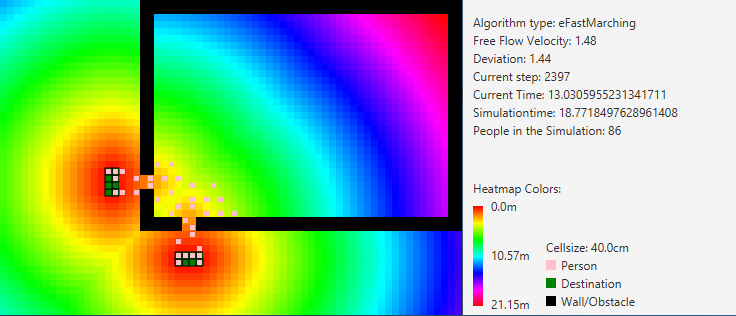
\includegraphics[width=\textwidth]{abbildungen/Evak1FMMitte.PNG}
	\end{minipage}
	\caption{Evakuierung eines Raumes mit 2 Türen (geringer Abstand), Dijkstra Algorithmus (links), Fast-Marching Algorithmus (rechts)}
	\label{fig:Evak2TNebeneinanderMinDijkstraFM}
\end{figure}

Die Abbildung \ref{fig:Evak2TNebeneinanderMinDijkstraFM} zeigt einen Ausschnitt der Simulation nach einer Simulationszeit von ca. $6s$. Wie zu erwarten ist, drängen alle Personen in die Ecke links unten. Dort bilden sich vor den Engstellen (Ausgängen) kleinere Staus. Die Evakuierungsdauer beträgt für die Simulation mit dem Dijkstra Algorithmus ca. $16,8s$. Da sich die Personen bei Verwendung des Fast Marching Algorithmus effizienter auf die Ziele zu bewegen, bilden sich etwas kleinere Staus an den Engstellen und die Evakuierungsdauer ist mit ca. $16,5s$ etwas kürzer.

\begin{figure}[!htb]
	\centering
	\begin{minipage}{.5\textwidth}
		\centering
		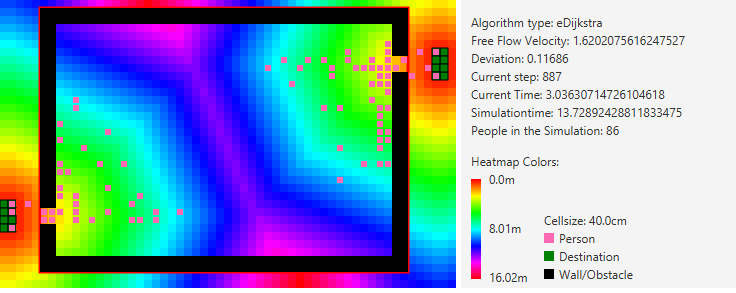
\includegraphics[width=\textwidth]{abbildungen/Evak2DMitte.PNG}
	\end{minipage}%
	\begin{minipage}{0.5\textwidth}
		\centering
		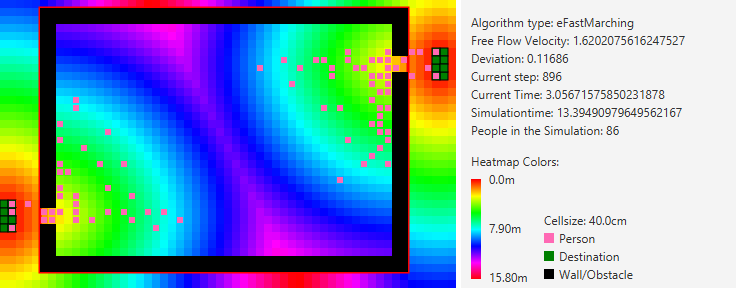
\includegraphics[width=\textwidth]{abbildungen/Evak2FMMitte.PNG}
	\end{minipage}
	\caption{Evakuierung eines Raumes mit 2 Türen (großer Abstand), Dijkstra Algorithmus (links), Fast-Marching Algorithmus (rechts)}
	\label{fig:Evak2TNebeneinanderMaxDijkstraFM}
	\end{figure}

Im Vergleich dazu zeigt die Abbildung \ref{fig:Evak2TNebeneinanderMaxDijkstraFM}   einen Ausschnitt der Simulation, in der die Ausgänge bzw. Ziele sehr weit voneinander entfernt gewählt wurden. Beide Algorithmen werden gegenübergestellt. In der Abbildung ist sofort zu sehen, dass sich in etwa die Hälfte der Personen (Personen deren Startposition in der entsprechenden Hälfte lag) auf die Ziele unten links und die andere Hälfte auf die Ziele oben rechts zubewegen. Die Heatmaps zeigen die entsprechende Entfernung an. Die maximale Entfernung, die eine Person von einer Tür haben kann, ist in der Simulation mit den nahe beieinander liegenden Türen fast doppelt so groß (ca. $28m$), wie in der Simulation in der die Türen weit voneinander entfernt sind (ca. $15m$).  \\
Die Evakuierungsdauer ist mit ca. $12,53s$ (Dijkstra) bzw. $12,6s$ (Fast-Marching) deutlich kürzer als im zuvor beschrieben Szenario (vgl. Abbildung \ref{fig:Evak2TNebeneinanderMinDijkstraFM}). Um diesen Zusammenhang weiter zu überprüfen, wurde eine zusätzliche Map mit deutlich mehr Personen im Raum angelegt. Die Positionen der Türen wurde nicht verändert. Da hierbei vor allem die Auswirkung der Position der Türen auf die Evakuierungsdauer ermittelt werden soll, wurde dieser zusätzliche Test nur auf Basis des Dijkstra Algorithmus durchgeführt. Die Implementierung der Simulation ermöglicht jedoch, diesen bei Bedarf auf Basis des Fast-Marching Algorithmus zu wiederholen.\\

\begin{figure}[!htb]
	\centering
	\begin{minipage}{.5\textwidth}
		\centering
		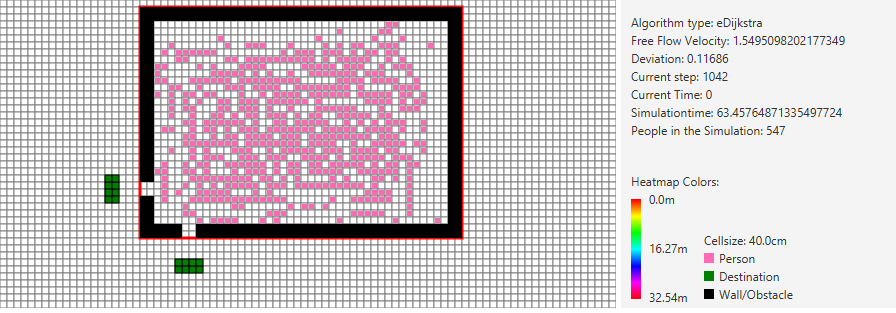
\includegraphics[width=\textwidth]{abbildungen/Evak2TMinDis2.png}
	\end{minipage}%
	\begin{minipage}{0.5\textwidth}
		\centering
		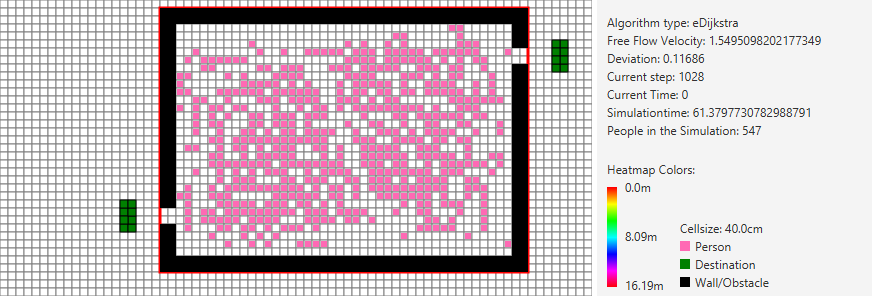
\includegraphics[width=\textwidth]{abbildungen/Evak2TMaxDis2.png}
	\end{minipage}
	\caption{Evakuierung eines Raumes mit 2 Türen, links: geringer Abstand zwischen den Türen, rechts: großer Abstand zwischen den Türen}
	\label{fig:Evak2TminmaxDis2}
\end{figure}

Abbildung \ref{fig:Evak2TminmaxDis2} zeigt die Aufteilung der $547$ Personen und die Positionen der Türen in den beiden Szenarien. 

\begin{figure}[!htb]
	\centering
	\begin{minipage}{.5\textwidth}
		\centering
		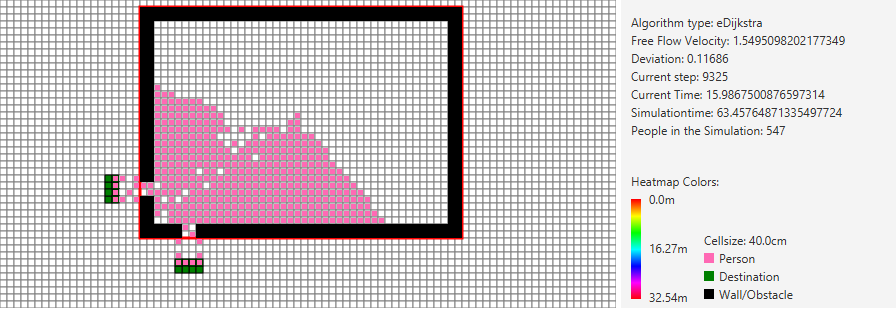
\includegraphics[width=\textwidth]{abbildungen/Evak2TMinDis2MITTE.png}
	\end{minipage}%
	\begin{minipage}{0.5\textwidth}
		\centering
		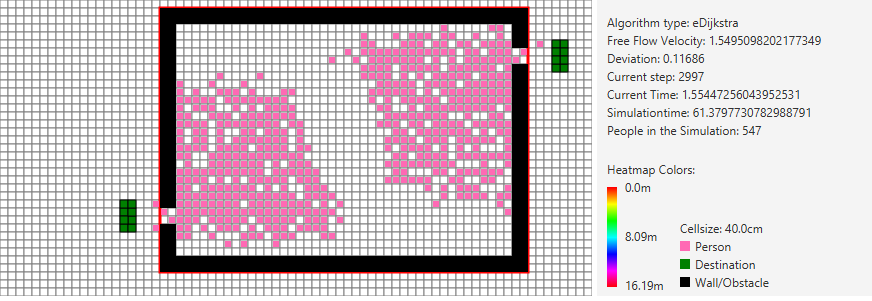
\includegraphics[width=\textwidth]{abbildungen/Evak2TMaxDis2MITTE.png}
	\end{minipage}
	\caption{Evakuierung eines Raumes mit 2 Türen (Ausschnitt der Simulation), links: geringer Abstand zwischen den Türen, rechts: großer Abstand zwischen den Türen}
	\label{fig:Evak2TminmaxDis2MITE}
\end{figure}

Die Abbildung \ref{fig:Evak2TminmaxDis2MITE} zeigt einen Ausschnitt der Simulation bei $15,97s$ (links) bzw. $1,55s$ (rechts). In beiden Abbildungen ist deutlich zu sehen, dass sich die Personen, aufgrund der hohen Personenanzahl, vor allen Türen stauen.

\begin{figure}[!htb]
	\centering
	\begin{minipage}{.5\textwidth}
		\centering
		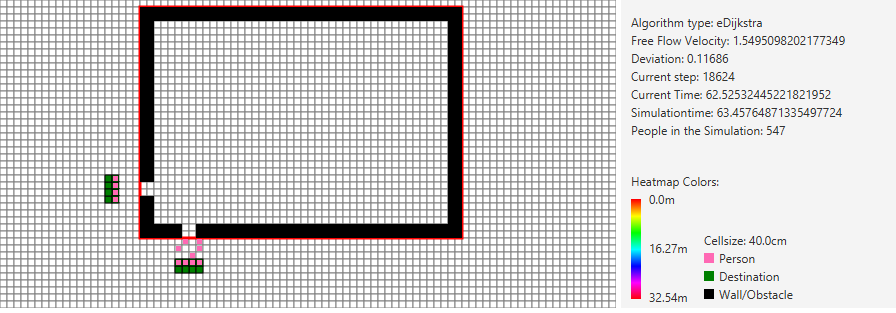
\includegraphics[width=\textwidth]{abbildungen/Evak2TMinDis2ENDE.png}
	\end{minipage}%
	\begin{minipage}{0.5\textwidth}
		\centering
		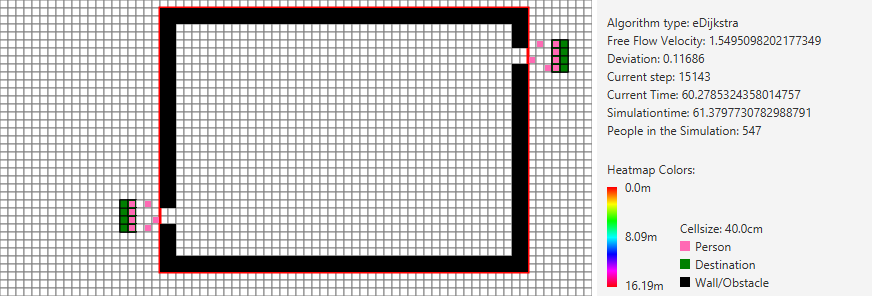
\includegraphics[width=\textwidth]{abbildungen/Evak2TMaxDis2ENDE.png}
	\end{minipage}
	\caption{Evakuierung eines Raumes mit 2 Türen (Ausschnitt: Ende der Evakuierung), links: geringer Abstand zwischen den Türen, rechts: großer Abstand zwischen den Türen}
	\label{fig:Evak2TminmaxDis2ENDE}
\end{figure}

Abschließend zeigt die Abbildung \ref{fig:Evak2TminmaxDis2ENDE} das Ende der Evakuierung der beiden Räume. Die Evakuierung eines Raumes, bei dem die Türen weit voneinander entfernt sind, verläuft mit einer Dauer von ca. $60,28s$ um ca. $2,3s$ schneller als die eines Raumes, bei dem die Türen nah beieinander liegen ($62,53s$). Durch eine höhere Anzahl an Personen, wirkt sich die Position der Türen somit nur noch sehr gering auf die Evakuierungsdauer aus. Hintergrund hierfür könnte die lange Wartezeit bzw. der große Stau vor den jeweiligen Türen sein. Da die Wartezeit der einzelnen Personen teilweise sehr hoch ist, wirkt sich der längere Weg bis zur Tür kaum auf die Evakuierungsdauer aus.
 
\paragraph{Fazit und Vergleich}


\subsubsection{Engstelle}
Anhand dieses Testszenarios soll ermittelt werden, welchen Einfluss das Variieren der Anzahl an Personen im Szenario auf die Simulationsdauer hat. Hierfür müssen die Personen einen $72\ m$ langen und $11,6\ m$ breiten Gang durchlaufen. Nach einer Länge von ca. $68\ m$ befindet sich eine $1,2\ m$ breite und $0,80\ m$ lange Engstelle.
Darüber hinaus wird die Personendichte in einem Messbereich (in den Abildungen rot hervorgehoben) vor der Engstelle gemessen und der Personengeschwindigkeit in einem Fundamentaldiagramm gegenübergestellt. Abbildung \ref{fig:engstelleMAP} zeigt das beschriebene Szenario. Für die Wegefindung wurde in diesem Testszenario der Dijkstra Algorithmus verwendet. 

\begin{figure}
\centering
\begin{minipage}{1\textwidth}
\centering
  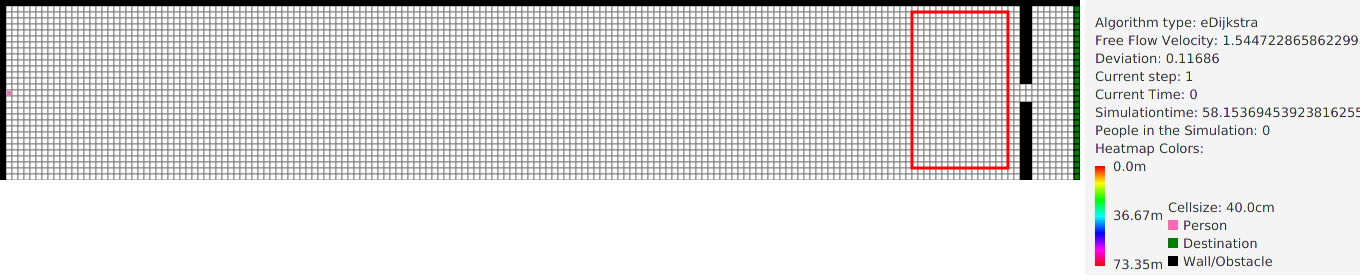
\includegraphics[width=1\linewidth]{abbildungen/engstelle/engstelleMAP.png}
\end{minipage}%
\\
\begin{minipage}{1\textwidth}
\centering
  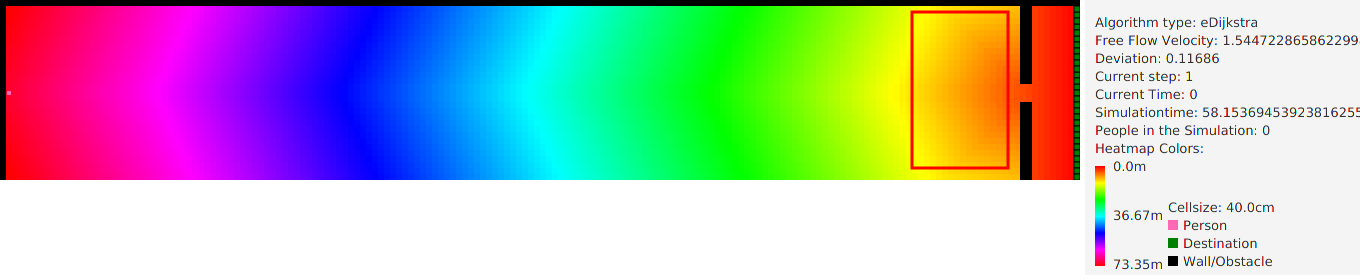
\includegraphics[width=1\linewidth]{abbildungen/engstelle/engstelleHEATMAP.png}
\end{minipage}
\caption{Darstellung der Karte als Cellmap (links) und Heatmap (rechts)}
\label{fig:engstelleMAP}
\end{figure}

Es es wurde zunächst nur eine Person eingefügt, um die Zeit, die für die Überwindung der Strecke benötigt wird zu ermitteln. Anschließend wurde der Test mit 10, 50, 100, 1000 und 2000 Personen wiederholt. Die unterschiedlichen Zeiten sind in der Tabelle \ref{tab:SimuZeitEngstelle} aufgeführt. Bis zu einer Personenzahl von $50$ liegen die Zeiten sehr nah beieinander. Die Simulation zeigt, dass die Anzahl der Personen zu gering bzw. die Engstelle breit genug ist, sodass sich die Personen nicht stauen. Bei einer Personenzahl von $100$ bilden sich erstmals leichte Staus, wodurch die Simulationszeit ($66,82 s$) um ca. $4\ s$ ansteigt.\\

\begin{table}[htpb]
	\centering
	\begin{tabular}{lll}
		Anzahl der Personen & Simulationszeit  &  Besonderheit\\ \hline
		$1$ Person & $58,15\ s$  &  Kein Stau vor der Engstelle\\ 
		$10$ Personen & $59,24\ s$  &  Kein Stau vor der Engstelle\\ 
		$50$ Personen & $62,83\ s$  &  Kein Stau vor der Engstelle\\ 
		$100$ Personen & $66,82\ s$  &  Leichter Stau vor der Engstelle\\ 
		$1000$ Personen & $189,95\ s$  &  Stau vor der Engstelle\\ 
		$2000$ Personen & $329,33\ s$  &  Großer Stau vor der Engstelle\\ 
 
	\end{tabular}
	\caption{Vergleich der unterschiedlichen Simulationszeiten abhängig von der Personenzahl}
	\label{tab:SimuZeitEngstelle}
\end{table}

Die Simulation mit einer Personenzahl von $1000$ zeigt zunächst, dass sich die unterschiedlichen Wunschgeschwindigkeiten der Personen aufgrund des langen Ganges stark auswirken. Schnellere Personen überholen langsamere, sodass nicht alle Personen gleichzeitig die Engstelle erreichen. Trotzdem ist die Anzahl der Personen zu groß bzw. die Engstelle zu schmal, sodass sich die Personen vor der Engstelle stauen. Beides ist in Abbildung \ref{fig:engstelle1000p} zu sehen. Dies wirkt sich deutlich auf die Simulationsdauer aus. Die Personendichte und die Personengeschwindigkeit im Messbereich sind im Fundamentaldiagramm (vgl. Abbildung \ref{fig:engstelle1000pFUNDA} gegenübergestellt. Zusätzlich wurde eine polinomische Trendlinie vierten Grades eingefügt. Im Fundamentaldiagramm ist lediglich der Zeitraum dargestellt, ab dem sich Personen im Messbereich befinden und bis die maximale Dichte erreicht ist. Es ist anzumerken, dass die Verteilung der Personen über den Messbereich nicht gleichmäßig ist. Zu Beginn stauen sich die Personen lediglich in einem Halbkreis um die Engstelle. Wenn die Personen den Messbereich wieder verlassen, also der Stau sich auflöst, verringert sich die Personendichte. Die Geschwindigkeit erhöht sich jedoch nicht signifikant. Dies ist in Abbildung \ref{fig:engstelle1000pFUNDAALL} dargestellt.

\begin{figure}
\centering
\begin{minipage}{1\textwidth}
\centering
  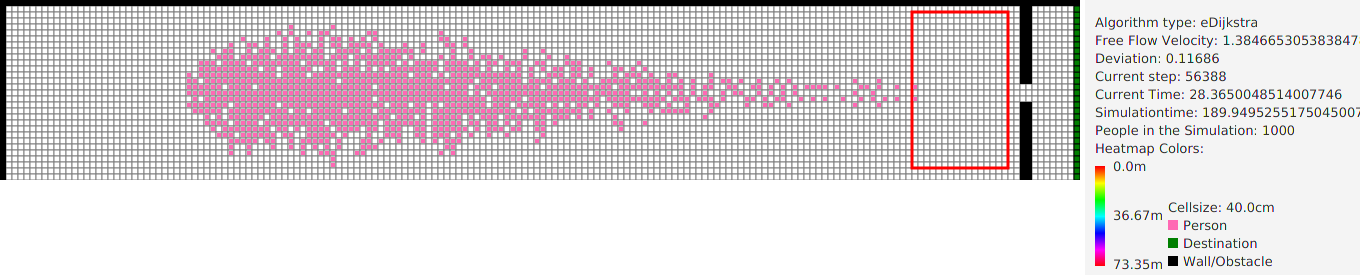
\includegraphics[width=1\linewidth]{abbildungen/engstelle/1000P/engstelle1000personenVORmessbereich.png}
\end{minipage}%
\\
\begin{minipage}{1\textwidth}
\centering
  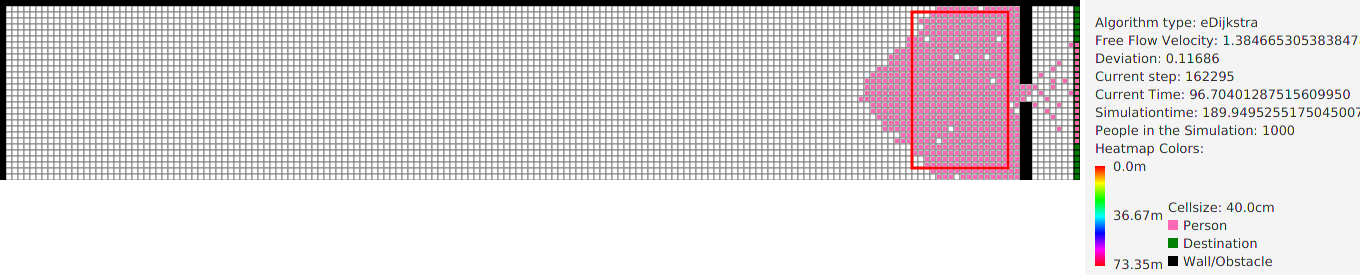
\includegraphics[width=1\linewidth]{abbildungen/engstelle/1000P/engstelle1000personenMAXmessbereich.png} 
 \end{minipage}
\caption{Ausschnitt aus der Simulation mit 1000 Personen, Verteilung der Personen aufgrund individueller Geschwindigkeit (links) und Bildung des Staus vor der Engstelle (rechts)}
\label{fig:engstelle1000p}
\end{figure}

\begin{figure}[ht]
	\centering
  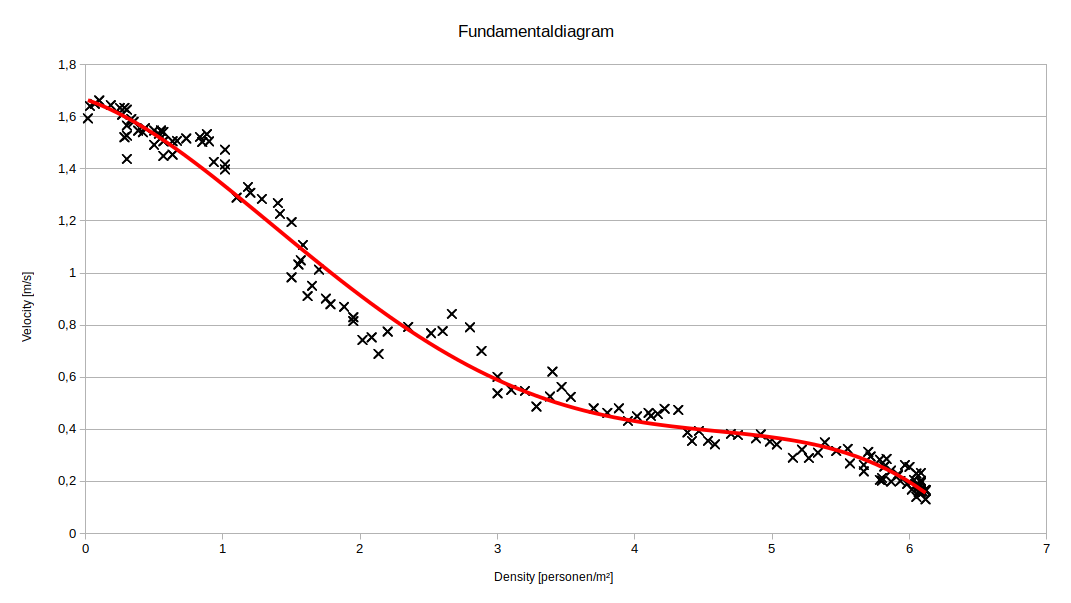
\includegraphics[width=\textwidth]{abbildungen/engstelle/1000P/fundamentalDiagram1000persons.png}
	\caption{Fundamentaldiagramm der Simulation mit 1000 Personen}
	\label{fig:engstelle1000pFUNDA}
\end{figure}

\begin{figure}[ht]
	\centering
  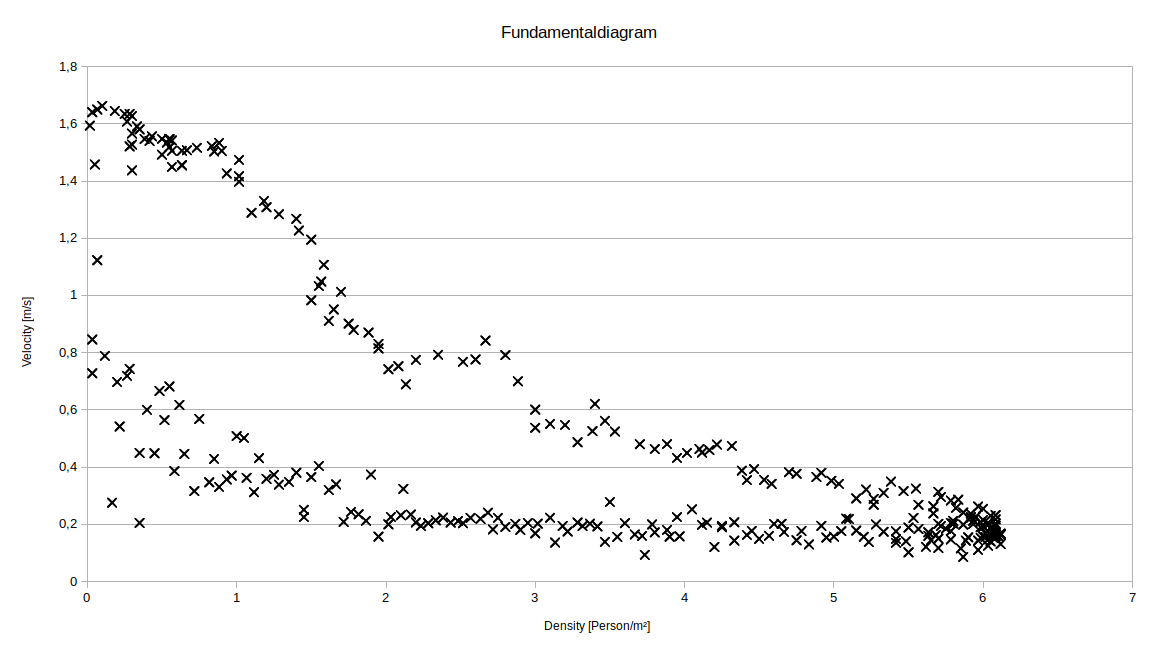
\includegraphics[width=\textwidth]{abbildungen/engstelle/1000P/fundamentalDiagram1000personsALLDATA.png}
	\caption{Fundamentaldiagramm der Simulation mit 1000 Personen (Ab Staubildung bis Ende des Staus)}
	\label{fig:engstelle1000pFUNDAALL}
\end{figure}

Im Vergleich dazu zeigt die Simulation mit 2000 Personen einen deutlichen Stau an der Engstelle. Die Simulationsdauer ist fast doppelt so groß wie bei der Simulation mit 1000 Personen. Die Bewegung der Personen und der Stau vor der Engstelle sind in Abbildung \ref{fig:engstelle2000p} dargestellt. Es wurden ebenfalls zwei Fundamentaldiagramme für den Messbereich erstellt. Abbildung \ref{fig:engstelle2000pFUNDA} zeigt das Fundamentaldiagramm für den Zeitraum zwischen dem ankommen der ersten Person im Messbereich und der maximalen Dichte im Messbereich. Abbildung \ref{fig:engstelle2000pFUNDAALL} zeigt das Fundamentaldiagramm bis zum Zeitpunkt, an dem die letzte Person den Messbereich verlassen hat. Ebenfalls ist zu sehen, dass sich die Geschwindigkeit trotz abnehmender Dichte nicht signifikant erhöht.\\

Zusammenfassend lässt sich feststellen, dass die Engstelle erst ab einer gewissen Personenzahl (in dieser Simulation 100 Personen) überhaupt Auswirkungen auf die Simulationsdauer hat. Bei geringer Personenzahl bleibt die Simulationsdauer annähernd gleich und variiert lediglich aufgrund der normalverteilten Wunschgeschwindigkeit der Personen. 

\begin{figure}
\centering
\begin{minipage}{1\textwidth}
\centering
  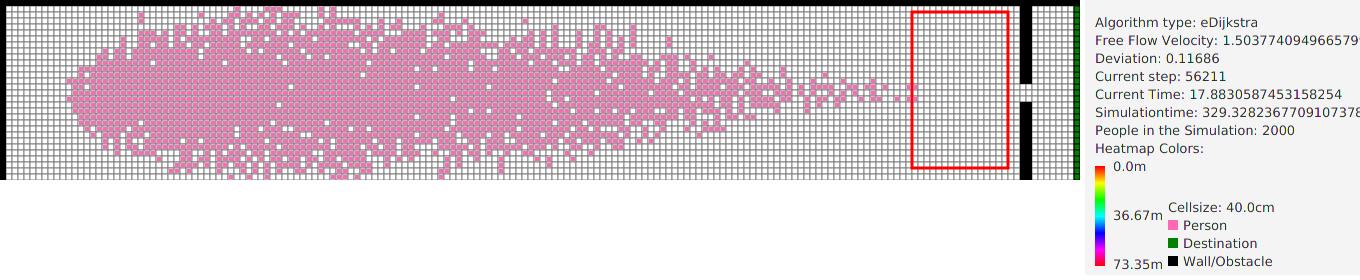
\includegraphics[width=1\linewidth]{abbildungen/engstelle/2000P/engstelle2000personenVORmessbereich.png}
\end{minipage}%
\\
\begin{minipage}{1\textwidth}
\centering
  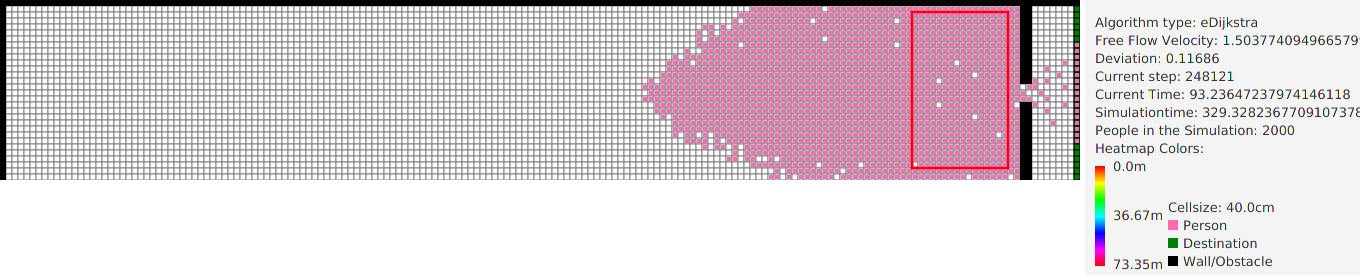
\includegraphics[width=1\linewidth]{abbildungen/engstelle/2000P/engstelle2000personenMAXmessbereich.png} 
 \end{minipage}
\caption{Ausschnitt aus der Simulation mit 2000 Personen, Verteilung der Personen aufgrund individueller Geschwindigkeit (links) und Bildung des Staus vor der Engstelle (rechts)}
\label{fig:engstelle2000p}
\end{figure}

\begin{figure}[ht]
	\centering
  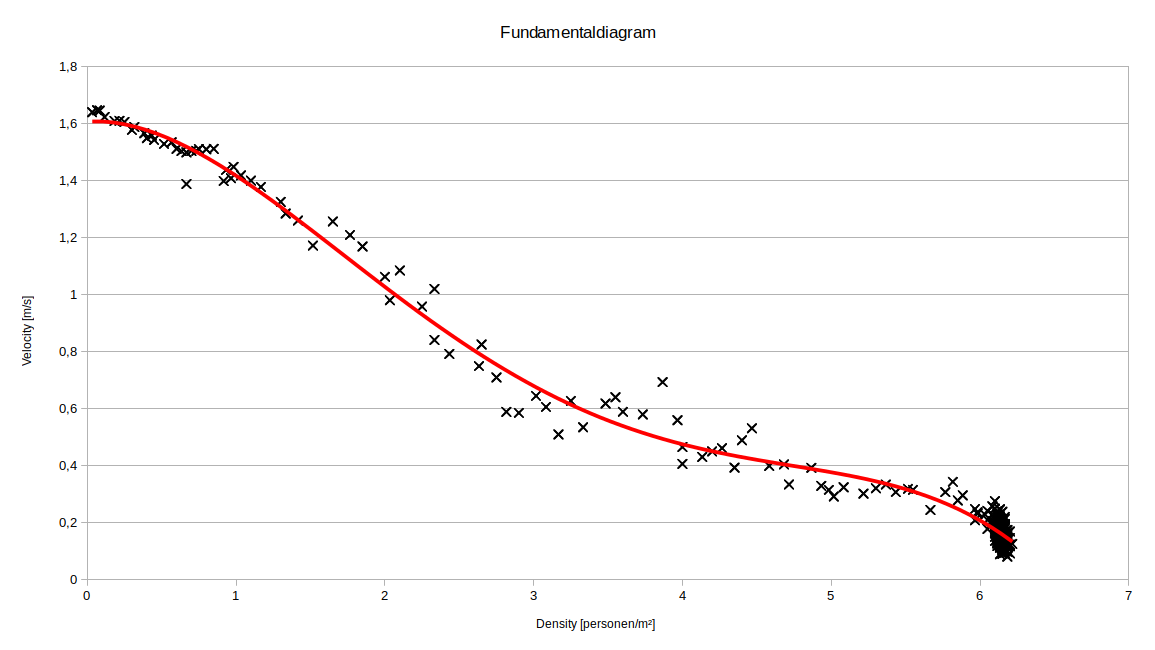
\includegraphics[width=\textwidth]{abbildungen/engstelle/2000P/fundamentalDiagram2000persons.png}
	\caption{Fundamentaldiagramm der Simulation mit 2000 Personen}
	\label{fig:engstelle2000pFUNDA}
\end{figure}

\begin{figure}[ht]
	\centering
  \includegraphics[width=\textwidth]{abbildungen/engstelle/2000P/fundamentalDiagram2000personsALLDATA.png}
	\caption{Fundamentaldiagramm der Simulation mit 2000 Personen (Ab Staubildung bis Ende des Staus)}
	\label{fig:engstelle2000pFUNDAALL}
\end{figure}


\subsection{Validation}

Zur Validation wurde der Rimea Test 4 mit unserer Software nachgebaut. Es wurde eine Karte mit $40cm$ großen Zellen erstellt, die $65$x$12m$ aufspannt.
Die Karte ist in Abbildung \ref{fig:rimea4:map} dargestellt. Der Nutzen wurde mit euklidischem Abstand berechnet, um Fehler zu vermeiden.

\begin{figure}
	\centering
	\includegraphics[width=0.7\linewidth]{abbildungen/fundamentaldiagramm/map}
	\caption{Karte für die Simulation des Rimea Test 4. Alle Zellen bis auf die Ziele der rechten Seite sind initial mit Personen befüllt.}
	\label{fig:rimea4:map}
\end{figure}

Damit sich die Personen gleichmäßig Verteilen und sich wie in einem endlosen Rundgang bewegen, wurde die Implementierung des Fields angepasst. Von Personen auf der rechten Seite vor dem Ziel werden wieder die Zellen der linken Seite betrachtet. Da es zunächst einige Artefakte bei diesem Sprung gab wurde sichergestellt, dass freie Zellen so wie das Personenpotential der jeweils anderen Seite betrachtet werden.

Um eine Änderung der Dichte zu erreichen, werden nach jeder Messung 30 zufällig verteilte Personen aus der Simulation entfernt. Messen wird jede Sekunde über das gesamte Feld durchgeführt.

Für das Ermitteln des Flusses wurde eine vertikale Linie über die ganze Höhe gewählt. Die Werte werden aber auf $1m$ normiert.

Die Simulation wurde durchgeführt und optisch kontrolliert ob die Personen gleichmäßig Verteil sind. Vier Bilder im Verlauf sind in Abbildung \ref{fig:rimea4:verlauf} aufgereiht. 

\begin{figure}
	\centering
	\includegraphics[width=0.7\linewidth]{abbildungen/fundamentaldiagramm/verlauf}
	\caption{Verlauf der Simulation mit dem Entfernen von Personen. Die Information zur Personenanzahl stimmt in diesem Fall nicht.}
	\label{fig:rimea4:verlauf}
\end{figure}

Das Fundamentaldiagramm der Simulation ist in Abbildung \ref{fig:rimea4:diagramm} zu sehen. Die Werte für die Personenabstoßung wurden kalibriert ($\mu$ 50.0 $a_p$ 1.0 $b_p$ 2). Vergleicht man es mit dem Fundamentaldiagramm von Weidmann (Abbildung \ref{fig:rimea4:weidman}) fällt auf, dass zwar der linke Teil bis zu einer Dichte von drei sehr gut passt, in der rechten Hälfte mit hoher Dichte danach allerdings die mittlere Geschwindigkeit wieder ansteigt. Dies steht im Widerspruch zu desn Ergebnissen aus dem Messexperiment. Die Abweichung findet sich auch im Flussdiagramm (Abbildung \ref{fig:rimea4:fluss}). Von kurz nach dem Beginn bis Sekunde $40$ (noch hohe Dichte) gibt es unerwartet den größten Fluss.

\begin{figure}
	\centering
	\includegraphics[width=0.7\linewidth]{abbildungen/fundamentaldiagramm/weidman}
	\caption{Fundamentaldiagramm nach Weidman. Quelle: U. Weidmann Transporttechnik der Fussgänger, Transporttechnische Eigenschaften des Fussgängerverkehrs (Literturauswertung) Schriftenreihe des IVT Nr. 90, Zweite, ergänzte Auflage, Zürich, März 1993 (109 Seiten)}
	\label{fig:rimea4:weidman}
\end{figure}

\begin{figure}
	\centering
	\includegraphics[width=0.7\linewidth]{abbildungen/fundamentaldiagramm/diagramm}
	\caption{Fundamentaldiagramm des Rimea Tests 4}
	\label{fig:rimea4:diagramm}
\end{figure}

\begin{figure}
	\centering
	\includegraphics[width=0.7\linewidth]{abbildungen/fundamentaldiagramm/fluss}
	\caption{Fluss des Rimea Test 4 über eine 1m vertikale Linie.}
	\label{fig:rimea4:fluss}
\end{figure}

Für bestimmte Dichten wurden keine Personen entnommen und geprüft ob die mittlere Geschwindigkeit konvergiert. Dies war der Fall und die Werte lagen auf der Kurve des vollen Fundamentaldiagramms (\ref{fig:rimea4:diagramm}). So kann ausgeschlossen werden, dass das Wegnehmen von Personen die Messwerte beeinflusst.

Für die nicht validen Ergebnisse ab einer Dichte größer drei wurden die Software und das Modell auf Fehler überprüft. Um die Suche einzuschränken wurde die Simulation ohne Personenpotential ausgeführt. Der Vergleich ist in Abbildung \ref{fig:rimea4:vergleich-ohnep} zu sehen. Das Personenpotential hat nur von Dichte eins bis ca. fünf einen Einfluss auf die Geschwindigkeit.
Entweder ist das Personenpotential falsch umgesetzt und müsste auch im Bereich für sehr hohen Dichten gelten oder die generelle Zuglogik ist für hohe Dichte falsch. Der Fluss der Simulation ohne Personenpotential sieht aber plausibel aus (Abbildung \ref{fig:rimea4:fluss-ohnep}).

\begin{figure}
	\centering
	\includegraphics[width=0.7\linewidth]{abbildungen/fundamentaldiagramm/vergleich-ohnep}
	\caption{Fundamentaldiagramm des Rimea Test 4 mit (orange) und ohne (blau) Personenpotential}
	\label{fig:rimea4:vergleich-ohnep}
\end{figure}



Eventuell liegt der Fehler auch an der Eigenschaft des zellulären Automaten. 
Ist eine Person bis auf eine Nachbarzelle komplett von Personen umringt, ist die Änderung des Nutzens durch das Personenpotential an beiden Stellen exakt gleich. So zieht die Person immer, wenn nur der Zellnutzen besser ist. Das könnte auch erklären, warum das Personenpotential bei hohen Dichten nicht greift. Möglicherweise ist die Zellgröße zu grob gewählt.

\begin{figure}
	\centering
	\includegraphics[width=0.7\linewidth]{abbildungen/fundamentaldiagramm/fluss-ohnep}
	\caption{Fluss im Rimea Test 4 ohne Personpotential}
	\label{fig:rimea4:fluss-ohnep}
\end{figure}

Leider können wir unsere Simulation wegen zu großer Abweichung im gerade interessanten Bereich mit hoher Dichte nicht validieren.
 
\section{Ausblick und Fazit}
Das Thema der Arbeit war die Bewegung von Personen in der Ebene zu simulieren. Zu Beginn wurde ein Java Programm implementiert, dass abhängig von Übergabeparameter und einer Karte, die das Feld mit Hindernissen beschreibt durchrechnet. Die Resultate wurden in eine Ausgabe Datei geschrieben. Diese konnte anschließend in einer Visualisierung dargestellt werden.

Die Personenbewegung wurde mit den Algorithmen Euklid, Dijkstra und Fast Marching berechnet und deren Resultate miteinander verglichen. Zudem wurde eine Personenabstoßung implementiert um  Ergebnisse zu erhalten, die näher an der Realität liegen. Zusätzlich wurde beschrieben wie die Zellgröße Einfluss auf die Ergebnisse nimmt. Zur Verifikation wurden mehrere Tests durchgeführt und dokumentiert. Anschließend ist eine Diskussion erfolgt, ob die implementierte Simulation relevant genug ist um die Realität zu einem gewissen Maße abbilden zu können.

Die Simulation bietet die Möglichkeit die Startvariablen und den Simulationsbereich frei zu definieren und dadurch verschiedenste Szenarien betrachten zu können. Eine Option ist es, die durchschnittliche individuelle Wunschgeschwindigkeit der Personen anzupassen, wenn beispielsweise die Passanten in der Situation einer gewissen Gruppe (z.B. Rentner) angehören. Um realistische Ergebnisse zu erhalten müssten hierfür nur die entsprechenden Werte vorher ermittelt werden. Eine eigene Auswertung der Daten wie in dem Messexperiment der ersten Studienarbeit bietet die Simulation nicht an. Dies könnte für eine Weiterführung des Projektes eine mögliche Erweiterung sein. Hinzukommt, dass keine Personen generiert werden, die sich absonderlich oder anders als die anderen Verhalten. Ein Beispiel wären Drängler sein. Diese könnten in Zukunft noch hinzugefügt werden.
%----------------------------------------------------------------------------------------
%\input{References}
\bibliography{Bibliographie}
\bibliographystyle{plain}

\end{document}
